\documentclass[11pt,a4paper]{article}
\usepackage[utf8]{inputenc}
\usepackage[T1]{fontenc}
\usepackage[brazil]{babel}
\usepackage{lmodern}
\usepackage{amsmath,amssymb,bm}
\usepackage{graphicx,booktabs,float,geometry,url,pdflscape,makecell}
\usepackage{tikz}
\usetikzlibrary{arrows.meta,positioning,shapes.geometric}
\usepackage[hidelinks]{hyperref}
\geometry{margin=2.2cm}
\providecommand{\versao}{sem versão}
\newcommand{\xib}{\bm\xi}
\newcommand{\refPfCe}{15,700\,\%}
\newcommand{\refNCe}{2\,148}
\newcommand{\lsNCe}{313}
\newcommand{\lsPfCe}{15,996\,\%}
\newcommand{\lsGanhoCe}{7}
\newcommand{\lsGanhoIsmcCe}{4,5}
\newcommand{\ismcNCe}{1\,397}
\newcommand{\refPfRa}{1,700\,\%}
\newcommand{\refNRa}{23\,129}
\newcommand{\lsNRa}{172}
\newcommand{\lsPfRa}{1,762\,\%}
\newcommand{\lsGanhoRa}{135}
\newcommand{\lsGanhoIsmcRa}{8,0}
\newcommand{\ismcNRa}{1\,375}
\newcommand{\refPfRb}{0,366\,\%}
\newcommand{\refNRb}{108\,781}
\newcommand{\lsNRb}{353}
\newcommand{\lsPfRb}{0,367\,\%}
\newcommand{\lsGanhoRb}{308}
\newcommand{\lsGanhoIsmcRb}{6,4}
\newcommand{\ismcNRb}{2\,270}
\newcommand{\hDirCe}{21}
\newcommand{\hMedDirCe}{19,8}
\newcommand{\hLsCe}{3,1}
\newcommand{\hIsmcCe}{13,9}
\newcommand{\efHLsCe}{7}
\newcommand{\efALsCe}{7}
\newcommand{\efAIsmcCe}{2}
\newcommand{\uDirCe}{35,6}
\newcommand{\uAmCe}{35,6}
\newcommand{\hDirRa}{445}
\newcommand{\hMedDirRa}{461,4}
\newcommand{\hLsRa}{3,2}
\newcommand{\hIsmcRa}{25,1}
\newcommand{\efHLsRa}{138}
\newcommand{\efALsRa}{141}
\newcommand{\efAIsmcRa}{19}
\newcommand{\uDirRa}{69,2}
\newcommand{\uAmRa}{65,8}
\newcommand{\hDirRb}{2\,061}
\newcommand{\hMedDirRb}{2\,084,6}
\newcommand{\hLsRb}{6,3}
\newcommand{\hIsmcRb}{39,7}
\newcommand{\efHLsRb}{327}
\newcommand{\efALsRb}{312}
\newcommand{\efAIsmcRb}{62}
\newcommand{\uDirRb}{68,2}
\newcommand{\uAmRb}{63,6}
\newcommand{\hIsmcTotal}{933}
\newcommand{\hIsmcBlocos}{961}
\newcommand{\hDirTotalCho}{2\,546}
\newcommand{\zDentro}{56}
\newcommand{\zSd}{0,62}
\newcommand{\icDentro}{43}
\newcommand{\icTotal}{43}
\newcommand{\zTotal}{56}
\newcommand{\viesParada}{0,03}
\newcommand{\viesParadaMin}{-2,1}
\newcommand{\viesParadaMax}{3,7}
\newcommand{\gimParedeIt}{1,8}
\newcommand{\gimCpuIt}{26}
\newcommand{\essIwMin}{14}
\newcommand{\essIwMax}{26}
\newcommand{\gimCpuItFermi}{37}
\newcommand{\lsIsmcMelhorRa}{7,5}
\newcommand{\lsIsmcMelhorRb}{5,1}
\newcommand{\lsIsmcMin}{3,6}
\newcommand{\lsIsmcMax}{8,3}
\newcommand{\zMaxTaludes}{0,75}
\newcommand{\formCeronCpu}{5,4}
\newcommand{\sgConfIguais}{20}
\newcommand{\sgConfTotal}{20}
\newcommand{\sgData}{20/11/2026 23:54}
\newcommand{\sgNmin}{1280}
\newcommand{\sgNmax}{2190}
\newcommand{\sgPares}{10\,180}
\newcommand{\sgDisc}{32}
\newcommand{\sgDiscSrm}{29}
\newcommand{\sgDiscGim}{3}
\newcommand{\sgDiscDist}{23}
\newcommand{\sgDiscCasoMin}{3}
\newcommand{\sgDiscCasoMax}{7}
\newcommand{\sgDiscFS}{0,0026}
\newcommand{\sgDiscG}{0,008}
\newcommand{\sgDiscGfs}{0,3}
\newcommand{\sgKmin}{2,6}
\newcommand{\sgKmax}{2,9}
\newcommand{\sgKperto}{2,67}
\newcommand{\sgDifMin}{$-$2,9}
\newcommand{\sgDifMax}{$+$0,2}
\newcommand{\sgZmax}{2,4}
\newcommand{\sgEdifMin}{0,8}
\newcommand{\sgEdifMax}{1,2}
\newcommand{\sgCovMin}{4,9}
\newcommand{\sgCovMax}{5,0}
\newcommand{\sgAbaixo}{5}
\newcommand{\sgCasos}{6}
\newcommand{\sgCampo}{0,56}
\newcommand{\sgDifAbsMax}{2,9}
\newcommand{\sgSubRaMin}{1,591}
\newcommand{\sgSubRaMax}{1,644}
\newcommand{\sgSubRbMin}{0,3511}
\newcommand{\sgSubRbMax}{0,3679}
\newcommand{\sgTgimMin}{57}
\newcommand{\sgTgimMax}{59}
\newcommand{\sgTsrmMin}{62}
\newcommand{\sgTsrmMax}{66}
\newcommand{\sgEcon}{9}
\newcommand{\sglN}{100}
\newcommand{\sglNGmin}{123}
\newcommand{\sglNGmax}{333}
\newcommand{\sglDifMin}{$-$1,7}
\newcommand{\sglDifMax}{$-$0,9}
\newcommand{\sglPrevMin}{$-$1,7}
\newcommand{\sglPrevMax}{$-$0,9}
\newcommand{\sglEdifMin}{0,2}
\newcommand{\sglEdifMax}{0,3}
\newcommand{\sglZmin}{3}
\newcommand{\sglZmax}{6}
\newcommand{\sglCovMin}{4,2}
\newcommand{\sglCovMax}{6,8}
\newcommand{\sglDcMin}{$+$0,004}
\newcommand{\sglDcMax}{$+$0,006}
\newcommand{\sglDcSdMin}{0,009}
\newcommand{\sglDcSdMax}{0,012}
\newcommand{\sglSmin}{0,06}
\newcommand{\sglSmax}{0,08}
\newcommand{\sglDfs}{0,04}
\newcommand{\sglNaSrmMin}{2,3}
\newcommand{\sglNaSrmMax}{2,7}
\newcommand{\sglNaGimMin}{2,6}
\newcommand{\sglNaGimMax}{3,0}
\newcommand{\sglCustoMin}{0}
\newcommand{\sglCustoMax}{$+$3}
\newcommand{\fgNRa}{7}
\newcommand{\fgBetaRa}{1,977}
\newcommand{\fnNRa}{243}
\newcommand{\fnBetaRa}{1,977}
\newcommand{\sUmRaMin}{1,630}
\newcommand{\sUmRaMax}{1,644}
\newcommand{\sOutRaMin}{1,669}
\newcommand{\sOutRaMax}{1,854}
\newcommand{\sJunRaMin}{1,718}
\newcommand{\sJunRaMax}{1,745}
\newcommand{\sPosRa}{1, 1, 1}
\newcommand{\fgNRb}{5}
\newcommand{\fgBetaRb}{2,463}
\newcommand{\fnNRb}{243}
\newcommand{\fnBetaRb}{2,466}
\newcommand{\sUmRbMin}{0,3511}
\newcommand{\sUmRbMax}{0,3679}
\newcommand{\sOutRbMin}{0,3412}
\newcommand{\sOutRbMax}{0,3772}
\newcommand{\sJunRbMin}{0,3516}
\newcommand{\sJunRbMax}{0,3656}
\newcommand{\sPosRb}{3, 3, 3}
\newcommand{\sgNRaMin}{1280}
\newcommand{\sgNRaMax}{1470}
\newcommand{\sgGaNmin}{2030}
\newcommand{\sgGaNmax}{2310}
\newcommand{\sgGaRaMin}{1,708}
\newcommand{\sgGaRaMax}{1,751}
\newcommand{\sgGaCovRaMin}{3,8}
\newcommand{\sgGaCovRaMax}{4,1}
\newcommand{\sgGaZRaMax}{0,5}
\newcommand{\sglGaPfRaMv}{1,724}
\newcommand{\sglGaNRaMv}{123}
\newcommand{\sglGaCovRaMv}{5,8}
\newcommand{\sglGaNcRaMv}{700}
\newcommand{\sglSNcRaMv}{480}
\newcommand{\sglGaPfRaGm}{1,724}
\newcommand{\sglGaNRaGm}{123}
\newcommand{\sglGaCovRaGm}{4,2}
\newcommand{\sglGaNcRaGm}{237}
\newcommand{\sglSNcRaGm}{172}
\newcommand{\sgGaRbMin}{0,3530}
\newcommand{\sgGaRbMax}{0,3586}
\newcommand{\sgGaCovRbMin}{4,6}
\newcommand{\sgGaCovRbMax}{4,8}
\newcommand{\sgGaZRbMax}{0,5}
\newcommand{\sglGaPfRbMv}{0,3514}
\newcommand{\sglGaNRbMv}{333}
\newcommand{\sglGaCovRbMv}{4,8}
\newcommand{\sglGaNcRbMv}{1\,148}
\newcommand{\sglSNcRbMv}{732}
\newcommand{\sglGaPfRbGm}{0,3545}
\newcommand{\sglGaNRbGm}{191}
\newcommand{\sglGaCovRbGm}{4,7}
\newcommand{\sglGaNcRbGm}{505}
\newcommand{\sglSNcRbGm}{353}
\newcommand{\sgGaZMax}{0,5}
\newcommand{\sglGaCustoMin}{38}
\newcommand{\sglGaCustoMax}{57}
\newcommand{\sglNaRazMin}{8}
\newcommand{\sglNaRazMax}{17}
\newcommand{\sglCovDoisMin}{21}
\newcommand{\sglCovDoisMax}{67}
\newcommand{\sglCovDoisGmMin}{21}
\newcommand{\sglCovDoisGmMax}{33}
\newcommand{\sglCurtErrMin}{16}
\newcommand{\sglCurtErrMax}{19}
\newcommand{\sglClRbMvCem}{69}
\newcommand{\sglClRbMvTodas}{88}
\newcommand{\sglCurtRbMvTodas}{39}
\newcommand{\sglClRbGmCem}{57}
\newcommand{\sglClRbGmTodas}{65}
\newcommand{\sglCurtRbGmTodas}{6}
\newcommand{\sgDiscFSmed}{0,0007}
\newcommand{\sgDistSrm}{20}
\newcommand{\sgDistGim}{3}
\newcommand{\sgDistP}{2 em 10\,000}
\newcommand{\ceaLsPf}{11,61\,\%}
\newcommand{\ceaLsLo}{10,49\,\%}
\newcommand{\ceaLsHi}{12,73\,\%}
\newcommand{\ceaLsCov}{4,9\,\%}
\newcommand{\ceaLsN}{153}
\newcommand{\ceaLsAn}{363}
\newcommand{\ceaLsZ}{$+$0,2}
\newcommand{\ceaForm}{4}
\newcommand{\ceaBeta}{1,152}
\newcommand{\ceaFormPf}{12,5\,\%}
\newcommand{\ceaMcN}{10\,000}
\newcommand{\ceaMcPf}{10,29\,\%}
\newcommand{\ceaMcPfEx}{10,32\,\%}
\newcommand{\ceaMcIc}{0,60\,\%}
\newcommand{\ceaMcRef}{993}
\newcommand{\ceaMcNovas}{3}
\newcommand{\ceaExMuda}{4}
\newcommand{\ceaExMax}{7,6}
\newcommand{\ceaMcSobe}{0,03}
\newcommand{\ceaMcZ}{$-$2,7}
\newcommand{\ceaGdetPz}{1,340}
\newcommand{\ceaGniveis}{1,401; 1,366; 1,351}
\newcommand{\ceaGnivelFim}{1,351}
\newcommand{\ceaGdetLa}{1,347}
\newcommand{\ceaGdetArt}{1,336}
\newcommand{\ceaGmedLa}{1,384}
\newcommand{\ceaGmedArt}{1,353}
\newcommand{\ceaPfArt}{11,50\,\%}
\newcommand{\ceaGvelho}{1,325}
\newcommand{\ceaZvelho}{$+$4,8}
\newcommand{\ceaLsDifPt}{0,1}
\newcommand{\ceaMcDifPt}{1,2}
\newcommand{\lmDirRaPf}{0,669\,\%}
\newcommand{\lmDirRaCov}{5,0\,\%}
\newcommand{\lmDirRaN}{60\,250}
\newcommand{\lmDirRaFal}{403}
\newcommand{\lmDirRaLo}{0,604\,\%}
\newcommand{\lmDirRaHi}{0,734\,\%}
\newcommand{\lmDirRaGmed}{2,093}
\newcommand{\lmDirRaRaz}{0,39}
\newcommand{\lmDirRaParN}{24\,000}
\newcommand{\lmDirRaParFl}{163}
\newcommand{\lmDirRaParFm}{408}
\newcommand{\lmDirRaParPm}{1,70\,\%}
\newcommand{\lmDirRaParRaz}{0,40}
\newcommand{\lmDirRaParErr}{0,02}
\newcommand{\lmDirRaSoL}{0}
\newcommand{\lmModoRaPe}{83,9}
\newcommand{\lmModoFRaPe}{87,1}
\newcommand{\lmModoRaFace}{15,7}
\newcommand{\lmModoFRaFace}{12,4}
\newcommand{\lmModoRaBase}{0,2}
\newcommand{\lmModoFRaBase}{0,5}
\newcommand{\lmDirRbPf}{0,113\,\%}
\newcommand{\lmDirRbCov}{33,3\,\%}
\newcommand{\lmDirRbN}{7\,930}
\newcommand{\lmDirRbFal}{9}
\newcommand{\lmDirRbLo}{0,039\,\%}
\newcommand{\lmDirRbHi}{0,188\,\%}
\newcommand{\lmDirRbGmed}{2,082}
\newcommand{\lmDirRbRaz}{0,31}
\newcommand{\lmDirRbParN}{7\,930}
\newcommand{\lmDirRbParFl}{9}
\newcommand{\lmDirRbParFm}{32}
\newcommand{\lmDirRbParPm}{0,40\,\%}
\newcommand{\lmDirRbParRaz}{0,28}
\newcommand{\lmDirRbParErr}{0,08}
\newcommand{\lmDirRbSoL}{0}
\newcommand{\lmModoRbPe}{88,5}
\newcommand{\lmModoFRbPe}{100,0}
\newcommand{\lmModoRbFace}{11,1}
\newcommand{\lmModoFRbFace}{0,0}
\newcommand{\lmModoRbBase}{0,3}
\newcommand{\lmModoFRbBase}{0,0}
\newcommand{\lmDirZPf}{3,91\,\%}
\newcommand{\lmDirZCov}{4,8\,\%}
\newcommand{\lmDirZN}{10\,460}
\newcommand{\lmDirZFal}{409}
\newcommand{\lmDirZLo}{3,54\,\%}
\newcommand{\lmDirZHi}{4,28\,\%}
\newcommand{\lmDirZGmed}{2,114}
\newcommand{\lmModoZPe}{74,8}
\newcommand{\lmModoFZPe}{74,1}
\newcommand{\lmModoZFace}{24,8}
\newcommand{\lmModoFZFace}{25,9}
\newcommand{\lmModoZBase}{0,3}
\newcommand{\lmModoFZBase}{0,0}
\newcommand{\lmZRazCeron}{0,71}
\newcommand{\lmZz}{$-$7,3}
\newcommand{\lmCeronPe}{80,8}
\newcommand{\lmCeronFace}{19,2}
\newcommand{\lmIsRaMin}{0,9261}
\newcommand{\lmIsRaMax}{0,9387}
\newcommand{\lmIsCovRaMin}{4,0}
\newcommand{\lmIsCovRaMax}{4,3}
\newcommand{\lmIsRazCincoRaMin}{0,54}
\newcommand{\lmIsRazCincoRaMax}{0,54}
\newcommand{\lmIsRazRaMin}{0,556}
\newcommand{\lmIsRazRaMax}{0,569}
\newcommand{\lmIsErrRaMax}{0,029}
\newcommand{\lmIsSoMRaMin}{108}
\newcommand{\lmIsSoMRaMax}{135}
\newcommand{\lmTodosRaMin}{0,9261}
\newcommand{\lmTodosRaMax}{0,9718}
\newcommand{\lmLsRaMin}{0,9275}
\newcommand{\lmLsRaMax}{0,9718}
\newcommand{\lmLsNaRaMin}{4,3}
\newcommand{\lmLsNaRaMax}{4,5}
\newcommand{\lmLsPerdRa}{0}
\newcommand{\lmLsRazRaMin}{0,547}
\newcommand{\lmLsRazRaMax}{0,552}
\newcommand{\lmLsDcRaMin}{$+$0,24}
\newcommand{\lmLsDcRaMax}{$+$0,24}
\newcommand{\lmLsDfsRaMin}{1,84}
\newcommand{\lmLsDfsRaMax}{1,86}
\newcommand{\lmSSrmRa}{0,077}
\newcommand{\lmBetaLaRaMv}{1,990}
\newcommand{\lmBetaMefRaMv}{1,977}
\newcommand{\lmCosRaMv}{0,9988}
\newcommand{\lmPhiRazRaMv}{0,97}
\newcommand{\lmBetaLaRaMc}{1,966}
\newcommand{\lmBetaMefRaMc}{1,956}
\newcommand{\lmCosRaMc}{0,9981}
\newcommand{\lmPhiRazRaMc}{0,98}
\newcommand{\lmDesAnRa}{$+$2,67}
\newcommand{\lmDesAnRaN}{1\,501}
\newcommand{\lmDesAnRaDp}{0,56}
\newcommand{\lmDesAnRaSp}{$+$2,67}
\newcommand{\lmGumAnRa}{1,076}
\newcommand{\lmPrevAnRa}{0,6667}
\newcommand{\lmPrevRazAnRa}{0,39}
\newcommand{\lmDesNyRa}{$+$1,87}
\newcommand{\lmDesNyRaN}{1\,911}
\newcommand{\lmDesNyRaDp}{0,45}
\newcommand{\lmDesNyRaSp}{$+$1,86}
\newcommand{\lmGumNyRa}{1,052}
\newcommand{\lmPrevNyRa}{0,9500}
\newcommand{\lmPrevRazNyRa}{0,56}
\newcommand{\lmObsNyRa}{0,9334}
\newcommand{\lmPtoDcRaMin}{$+$0,005}
\newcommand{\lmPtoDcRaMax}{$+$0,016}
\newcommand{\lmPtoFsRaMax}{0,12}
\newcommand{\lmIsRbMin}{0,1446}
\newcommand{\lmIsRbMax}{0,1512}
\newcommand{\lmIsCovRbMin}{4,9}
\newcommand{\lmIsCovRbMax}{5,7}
\newcommand{\lmIsRazCincoRbMin}{0,41}
\newcommand{\lmIsRazCincoRbMax}{0,43}
\newcommand{\lmIsRazRbMin}{0,414}
\newcommand{\lmIsRazRbMax}{0,436}
\newcommand{\lmIsErrRbMax}{0,025}
\newcommand{\lmIsSoMRbMin}{184}
\newcommand{\lmIsSoMRbMax}{237}
\newcommand{\lmTodosRbMin}{0,1446}
\newcommand{\lmTodosRbMax}{0,1512}
\newcommand{\lmLsRbMin}{0,1450}
\newcommand{\lmLsRbMax}{0,1507}
\newcommand{\lmLsNaRbMin}{4,6}
\newcommand{\lmLsNaRbMax}{4,8}
\newcommand{\lmLsPerdRb}{0}
\newcommand{\lmLsRazRbMin}{0,411}
\newcommand{\lmLsRazRbMax}{0,414}
\newcommand{\lmLsDcRbMin}{$+$0,30}
\newcommand{\lmLsDcRbMax}{$+$0,31}
\newcommand{\lmLsDfsRbMin}{1,79}
\newcommand{\lmLsDfsRbMax}{1,94}
\newcommand{\lmSSrmRb}{0,060}
\newcommand{\lmBetaLaRbMv}{2,484}
\newcommand{\lmBetaMefRbMv}{2,466}
\newcommand{\lmCosRbMv}{0,9981}
\newcommand{\lmPhiRazRbMv}{0,95}
\newcommand{\lmBetaLaRbMc}{2,454}
\newcommand{\lmBetaMefRbMc}{2,440}
\newcommand{\lmCosRbMc}{0,9979}
\newcommand{\lmPhiRazRbMc}{0,96}
\newcommand{\lmDesAnRb}{$+$2,58}
\newcommand{\lmDesAnRbN}{105}
\newcommand{\lmDesAnRbDp}{0,41}
\newcommand{\lmDesAnRbSp}{$+$2,58}
\newcommand{\lmGumAnRb}{1,065}
\newcommand{\lmPrevAnRb}{0,0945}
\newcommand{\lmPrevRazAnRb}{0,26}
\newcommand{\lmDesNyRb}{$+$1,80}
\newcommand{\lmDesNyRbN}{3\,310}
\newcommand{\lmDesNyRbDp}{0,40}
\newcommand{\lmDesNyRbSp}{$+$1,84}
\newcommand{\lmGumNyRb}{1,046}
\newcommand{\lmPrevNyRb}{0,1391}
\newcommand{\lmPrevRazNyRb}{0,38}
\newcommand{\lmObsNyRb}{0,1494}
\newcommand{\lmPtoDcRbMin}{$+$0,020}
\newcommand{\lmPtoDcRbMax}{$+$0,025}
\newcommand{\lmPtoFsRbMax}{0,15}
\newcommand{\lmPtoFsMax}{0,15}
\newcommand{\lmPtoDcMin}{$+$0,005}
\newcommand{\lmPtoDcMax}{$+$0,025}
\newcommand{\lmBandaAnMin}{$+$2,5}
\newcommand{\lmBandaAnMax}{$+$2,9}
\newcommand{\lmBandaNyMin}{$+$1,7}
\newcommand{\lmBandaNyMax}{$+$1,9}
\newcommand{\lmDet}{$-$0,10}
\newcommand{\lmFsDetLa}{1,2032}
\newcommand{\lmFsDetMef}{1,2044}
\newcommand{\lmAcima}{todos}
\newcommand{\lmGradeAn}{$-$0,89}
\newcommand{\lmGradeAnDp}{0,16}
\newcommand{\lmGradeAnN}{400}
\newcommand{\lmGradeAnUm}{$+$1,84}
\newcommand{\lmGradeAnDois}{$+$2,75}
\newcommand{\lmGradeNy}{$-$0,38}
\newcommand{\lmGradeNyDp}{0,10}
\newcommand{\lmGradeNyN}{37}
\newcommand{\lmGradeNyUm}{$+$1,35}
\newcommand{\lmGradeNyDois}{$+$1,74}
\newcommand{\lmGradeNyFsMin}{0,75}
\newcommand{\lmGradeNyFsMax}{1,07}
\newcommand{\lmGradeAnFsMin}{0,94}
\newcommand{\lmGradeAnFsMax}{1,44}
\newcommand{\lmZfator}{1,024}
\newcommand{\lmZprev}{4,70\,\%}
\newcommand{\lmZfatorCeron}{1,046}
\newcommand{\lmZmef}{7,40\,\%}
\newcommand{\lmZmefLo}{6,81\,\%}
\newcommand{\lmZmefHi}{8,00\,\%}
\newcommand{\lmZrazMef}{0,53}
\newcommand{\lmZrazMefErr}{0,03}
\newcommand{\lmZprevV}{4,78\,\%}
\newcommand{\lmZprevVLo}{4,37\,\%}
\newcommand{\lmZprevVHi}{5,20\,\%}
\newcommand{\lmZprevVraz}{0,65}
\newcommand{\lmZchoFig}{6,62\,\%}
\newcommand{\lnyN}{1\,500}
\newcommand{\lnyFal}{7}
\newcommand{\lnyPf}{0,47\,\%}
\newcommand{\lnyPfLo}{0,12\,\%}
\newcommand{\lnyPfHi}{0,81\,\%}
\newcommand{\lnyPfIs}{0,93\,\%}
\newcommand{\lnyZis}{$-$1,9}
\newcommand{\lnyEsp}{14}
\newcommand{\lnyFalB}{18}
\newcommand{\lnyPfB}{1,20\,\%}
\newcommand{\lnyPfIsB}{1,77\,\%}
\newcommand{\lanPfB}{1,33\,\%}
\newcommand{\lnyZisB}{$-$1,6}
\newcommand{\lnyRazMin}{1,11}
\newcommand{\lnyRazMax}{1,22}
\newcommand{\lnyZmin}{1,1}
\newcommand{\lnyZmax}{4,3}
\newcommand{\lisRazMin}{1,18}
\newcommand{\lisRazMax}{1,22}
\newcommand{\lnyIsMin}{0,91}
\newcommand{\lnyIsMax}{1,02}
\newcommand{\lnyMed}{$-$3,8}
\newcommand{\lnyQvc}{$-$3,9}
\newcommand{\lnyQcinco}{$-$0,9}
\newcommand{\lnyQum}{$+$1,3}
\newcommand{\lnyLg}{$-$3,9}
\newcommand{\lnyLgErr}{0,9}
\newcommand{\lnyLgZ}{4,3}
\newcommand{\lmefRazMin}{1,01}
\newcommand{\lmefRazMax}{1,06}

\title{Comparação dos métodos de confiabilidade:\\ Monte Carlo direto, ISMC e line sampling\\
\large Cho ($r = -0{,}5$ e $-0{,}7$), rebaixamento do Ceron e a viga}
\author{Diogo Cecílio}
\date{20/11/2026 --- versão \versao}
\begin{document}
\maketitle
\begin{abstract}
Reunimos, com os dados de 20/11/2026, todos os resultados de probabilidade de falha dos três problemas de talude e da
viga, por três métodos: o Monte Carlo direto (a referência), a amostragem por importância centrada no ponto de projeto
do FORM (ISMC) e o line sampling (LS) na direção do FORM. A medida comum é o número de análises do MEF para CoV de 5\,\%,
contando o FORM. O line sampling na direção do FORM modal com todos os modos foi o mais barato nos três taludes, sem viés
detectado: \lsNCe{} análises no Ceron com a água antiga (direto: \refNCe; melhor ISMC: \ismcNCe), \lsNRa{} no Cho com $r = -0{,}5$ (direto:
\refNRa; ISMC: \ismcNRa) e \lsNRb{} no Cho com $r = -0{,}7$ (direto: \refNRb; ISMC: \ismcNRb). Na viga, que não tem gradiente modal, o line
sampling na direção do FORM adjunto precisou de 92 (direto: 18\,666). Os dados das comparações com o direto estão completos: as
ISMC da etapa 3b chegaram ao CoV de 5\,\% em todas as sementes e todas as direções do line sampling terminaram; o line
sampling ainda tem uma semente só.

Para comparar os métodos de outras formas, acrescentamos: o tempo de CPU (o line sampling modal dá CoV de 5\,\% com
\hLsRb{} h$\cdot$núcleo no Cho com $r = -0{,}7$, contra \hIsmcRb{} da melhor ISMC e \hDirRb{} do direto); as iterações
do FORM; a convergência do CoV com $1/\sqrt{n}$ e a eficiência relativa (figura de mérito); os pesos e o tamanho efetivo
da amostra da ISMC; a busca de cada linha do line sampling (2 a 3 análises por linha, quase sem bissecção); e o CoV
estimado contra o observado entre sementes, com a cobertura dos intervalos (\icDentro{} de \icTotal{} intervalos da
ISMC contêm a $P_f$ do direto).

Duas comparações novas. (1) O SRM contra o GIM com uma semente só, pareada: as mesmas realizações da ISMC da semente 21
e as mesmas linhas do line sampling da semente 7 (Seção~\ref{sec:pareado}; o GIM ainda roda no fermi, e a ISMC dele é
parcial, com \sgNmin{} a \sgNmax{} realizações por caso). As $P_f$ diferem no máximo \sgDifAbsMax\,\%, com o GIM em
geral um pouco abaixo e sempre dentro do CoV de cada estimativa: na ISMC, só por realizações limítrofes
($|\mathrm{FS} - 1| \le$ \sgDiscFS); no line sampling, por um deslocamento pequeno do ponto em que cada linha entra na
falha. O GIM custa \sgEcon\,\% menos por análise (no line sampling, com mais análises por linha, o custo empata); a
análise limite do Ceron nos mesmos casos ainda está no fermi. (2) O Ceron com a água do
artigo (Seção~\ref{sec:ceronagua}): o line sampling do MEF dá \ceaLsPf, contra \ceaPfArt{} do artigo. As outras linhas
do Ceron são do modelo de água antigo.
\end{abstract}
\tableofcontents

\section{Os dados}
\begin{itemize}
  \item \textbf{Monte Carlo direto:} completo nos quatro problemas (Tabela~\ref{tab:ref}).
  \item \textbf{ISMC da etapa 3b} (Cho, no fermi): 5 sementes por centro, com parada
    pelo CoV de 5\,\%: todas as 30 sementes pararam com CoV entre 4,6 e 5,0\,\% (1160 a 2990 realizações cada); a
    ISMC de cada centro junta as 5 sementes (CoV de 2,2\,\%), e o custo para CoV de 5\,\% vem do CoV combinado.
    No Ceron, as duas ISMC (1000 realizações cada) terminaram.
  \item \textbf{Line sampling:} 100 linhas por direção e uma semente só (a 7), no PC. As direções do FORM modal com 2000
    termos e do FORM numérico com $M = 20$ (Cho) e as três do Ceron terminaram. O CoV vem da dispersão das próprias
    linhas e ainda não foi conferido entre sementes.
  \item \textbf{Viga:} MC direto e ISMC completos (relatório da viga); o line sampling e o FORM adjunto rodaram nas seções
    16 e 17 do código em Mathematica (\path{viga_mathematica/codigo/viga_FORM5_AI200.txt}), ainda fora do relatório da
    viga.
  \item \textbf{SRM $\times$ GIM, pareado} (Seção~\ref{sec:pareado}): a campanha \texttt{etapa3b\_gim} do fermi,
    \textbf{ainda rodando} (dados de \sgData): a ISMC da semente 21 nos três centros e o line sampling da semente 7 nas
    duas direções, com o GIM no lugar do SRM. \textbf{Parcial} na ISMC: \sgNmin{} a \sgNmax{} realizações por caso (a
    campanha vai a pelo menos 2000); no line sampling, as \sglN{} linhas do SRM já têm todas o par no GIM. A análise
    limite do Ceron (2025) nos mesmos casos também está no fermi; aqui entra só o piloto local.
  \item \textbf{Ceron com a água do artigo} (Seção~\ref{sec:ceronagua}): o line sampling do MEF (no PC) e o MC de
    10\,000 realizações pela análise limite em Python. As outras linhas do Ceron são do modelo de água antigo.
\end{itemize}
Tudo sai do \path{gera_dados.py}, nesta pasta, que lê os resultados em \path{~/projects/runs}: rodar de novo atualiza as
figuras e as tabelas (\path{gera_relatorio.sh}).

\section{Os métodos em uma página}
A formulação está em \path{docs/confiabilidade_campos/formulacao} (Seções do Monte Carlo, da amostragem por importância,
do FORM e do line sampling). Em resumo, no espaço $\mathbb{Y}$ dos coeficientes $\xib \sim N(\bm 0, I)$ da expansão de
Karhunen--Loève:
\begin{itemize}
  \item \textbf{Monte Carlo direto:} $\hat P_f = \frac1N\sum I(\xib_\ell)$. Não depende de nada, mas precisa de
    $(1 - P_f)/(0{,}05^2 P_f)$ realizações para CoV de 5\,\%: 100\,000 com $P_f = 0{,}4\,\%$.
  \item \textbf{ISMC:} sorteia em torno do ponto de projeto, $\xib \sim N(\xib^*, I)$, e corrige cada amostra pelo peso
    exato $w = e^{-\xib^*\cdot\xib + |\xib^*|^2/2}$.
  \item \textbf{Line sampling:} sorteia linhas paralelas à direção $\bm e = \xib^*/\beta$ e calcula exatamente a
    probabilidade de falha de cada uma, $p_\ell = \Phi(-\nu_\ell)$, em que $\nu_\ell$ é onde a linha entra na falha
    (Figura~\ref{fig:esquema}). Só a curvatura da superfície de falha e os modos que a direção não vê entram na
    variância.
\end{itemize}
\begin{figure}[H]\centering
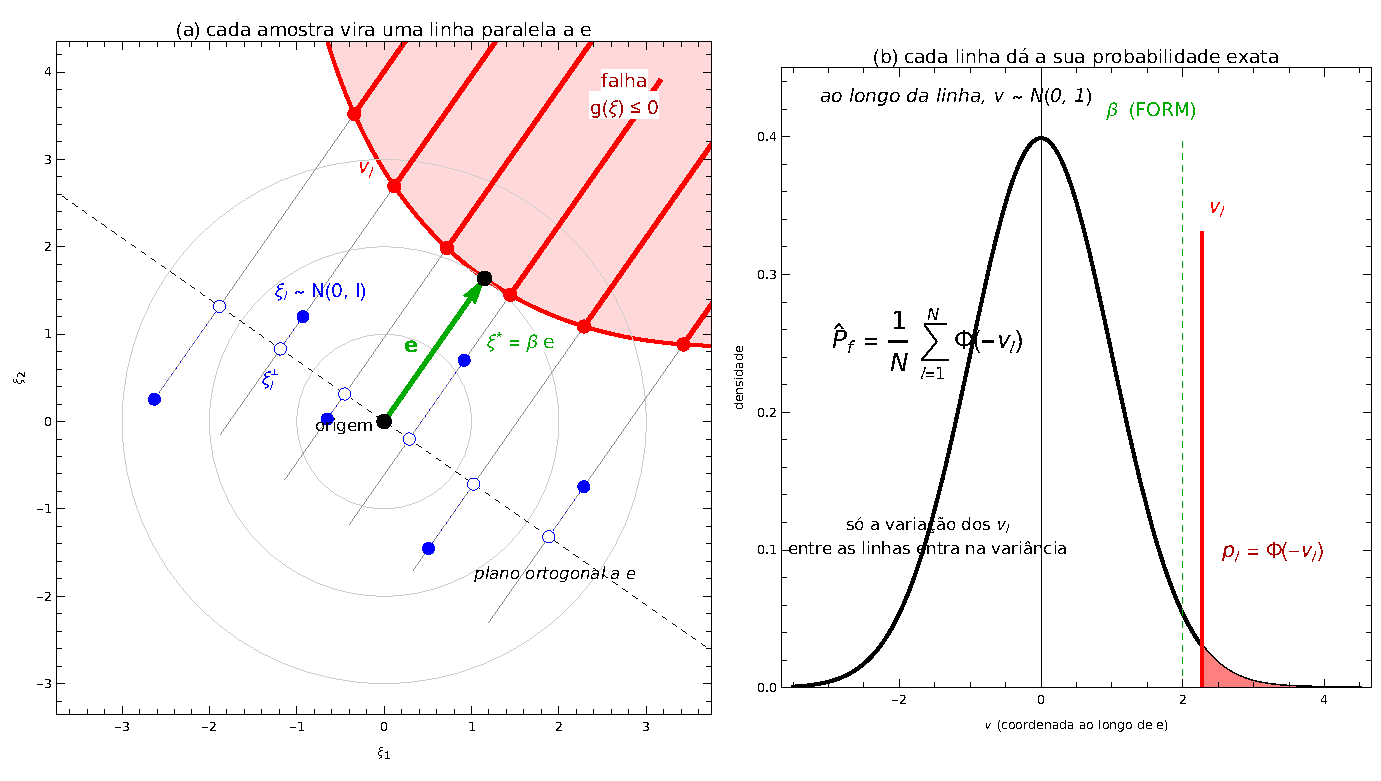
\includegraphics[width=\textwidth]{figs/ls_esquema.pdf}
\caption{O line sampling (da formulação). (a) Cada amostra é projetada no plano ortogonal a $\bm e$, e a linha que passa
pela projeção entra na falha em $\nu_\ell$. (b) Ao longo da linha, $\nu \sim N(0, 1)$, e a probabilidade de falha da
linha é a cauda $\Phi(-\nu_\ell)$.}\label{fig:esquema}
\end{figure}

\begin{figure}[H]\centering
\resizebox{\textwidth}{!}{%
\begin{tikzpicture}[node distance=6mm and 4mm, every node/.style={font=\footnotesize},
  caixa/.style={draw, rounded corners, align=center, minimum height=12mm, text width=29mm, fill=blue!6},
  cinza/.style={draw, rounded corners, align=center, minimum height=12mm, text width=29mm, fill=orange!10},
  seta/.style={-{Stealth[length=2.5mm]}, thick}]
\node[caixa] (form) {\textbf{FORM modal}\\ todos os modos\\ 3 a 7 análises};
\node[caixa, right=of form] (dir) {\textbf{direção}\\ $\bm e = \xib^*/\beta$\\ e a inclinação $s$ (2 análises)};
\node[caixa, right=of dir] (lin) {\textbf{$N$ linhas}\\ $\nu_\ell$ pela secante\\ 2 a 3 análises cada};
\node[caixa, right=of lin] (pf) {\textbf{$\hat P_f = \frac1N\sum\Phi(-\nu_\ell)$}\\ CoV pela dispersão\\ dos $p_\ell$};
\draw[seta] (form) -- (dir); \draw[seta] (dir) -- (lin); \draw[seta] (lin) -- (pf);
\node[cinza, below=of form] (form2) {\textbf{FORM}\\ (numérico ou modal)};
\node[cinza, right=of form2] (cen) {\textbf{centro}\\ $\xib^*$};
\node[cinza, right=of cen] (amo) {\textbf{$N$ amostras}\\ $\xib \sim N(\xib^*, I)$\\ 1 análise cada};
\node[cinza, right=of amo] (pf2) {\textbf{$\hat P_f = \frac1N\sum I w$}\\ peso exato};
\draw[seta] (form2) -- (cen); \draw[seta] (cen) -- (amo); \draw[seta] (amo) -- (pf2);
\node[left=2mm of form, rotate=90, anchor=south] {\textbf{LS}};
\node[left=2mm of form2, rotate=90, anchor=south] {\textbf{ISMC}};
\end{tikzpicture}}
\caption{Os dois métodos com o FORM, lado a lado. A diferença está no que se faz com o ponto de projeto: a ISMC o usa
como centro e sorteia pontos (cada um vale 0 ou $w$); o line sampling o usa como direção e sorteia linhas (cada uma vale
a probabilidade exata ao longo dela, entre 0 e 1).}\label{fig:fluxo}
\end{figure}

\section{Os problemas, as referências e os FORM}
\begin{itemize}
  \item \textbf{Cho (2010), Exemplo 2:} talude seco, $c'$ e $\varphi'$ lognormais com correlação cruzada $r = -0{,}5$ ou
    $-0{,}7$, SRM com refinamento adaptativo (\texttt{tri2} e 4 níveis). As ISMC e o line sampling usam o campo de Nyström
    de 2000 modos por campo (a etapa 3b); os diretos, a KL analítica (as mesmas estatísticas).
  \item \textbf{Ceron (2025), rebaixamento rápido:} $c'$, $\varphi'$ e $k_s$ aleatórios, transiente e GIM (o fator
    $\Gamma$), com 2000 modos por campo. As linhas ``Ceron (água antiga)'' das tabelas e das figuras usam o modelo de
    água antigo (o rebaixamento em 0,1\,h, com o transiente; $P_f$ do direto de \refPfCe); com a água do artigo, o
    line sampling do MEF dá \ceaLsPf{} (Seção~\ref{sec:ceronagua}).
  \item \textbf{Viga:} módulo de elasticidade lognormal (200 modos de Nyström), falha pela flecha no meio do vão.
\end{itemize}

% gerado por gera_dados.py: nao editar a mao
\begin{table}[H]\centering\small
\caption{As referências: o Monte Carlo direto de cada problema. O custo para CoV de 5\,\% é $(1 - P_f)/(0{,}05^2 P_f)$.}\label{tab:ref}
\begin{tabular}{lrrrrr}\toprule
problema & $N$ & falhas & $P_f$ & CoV & $N$ p/ CoV 5\,\% \\\midrule
Ceron, rebaixamento & 2\,000 & 314 & 15,700\,\% & 5,2\,\% & 2\,148 \\
Cho, $r = -0{,}5$ & 24\,000 & 408 & 1,700\,\% & 4,9\,\% & 23\,129 \\
Cho, $r = -0{,}7$ & 110\,000 & 403 & 0,366\,\% & 5,0\,\% & 108\,781 \\
viga (Mathematica) & 50\,000 & 1049 & 2,098\,\% & 3,1\,\% & 18\,666 \\
\bottomrule\end{tabular}\end{table}

\begin{table}[H]\centering\small
\caption{Os FORM que dão os centros da ISMC e as direções do line sampling. ``Numérico'': diferenças centrais ($4M + 1$ análises por iteração no Cho, $6M + 1$ no Ceron); ``modal'': o gradiente pela projeção modal do GIM (1 análise por iteração).}\label{tab:form}
\begin{tabular}{llrrrr}\toprule
problema & FORM & $\beta$ & $\Phi(-\beta)$ & análises & usado em \\\midrule
Ceron, rebaixamento & FORM $M = 20$, numérico & 1,153 & 12,45\,\% & 363 & ISMC, LS \\
Ceron, rebaixamento & FORM $M = 20$, modal & 1,205 & 11,41\,\% & 3 & ISMC, LS \\
Ceron, rebaixamento & FORM $M = 2000$, modal & 0,982 & 16,30\,\% & 3 & LS \\
Cho, $r = -0{,}5$ & FORM $M = 20$, numérico & 1,977 & 2,40\,\% & 243 & ISMC, LS \\
Cho, $r = -0{,}5$ & FORM $M = 100$, numérico & 1,956 & 2,52\,\% & 1203 & ISMC \\
Cho, $r = -0{,}5$ & FORM $M = 20$, modal & 2,003 & 2,26\,\% & 10 & ISMC \\
Cho, $r = -0{,}5$ & FORM $M = 2000$, modal & 1,977 & 2,40\,\% & 7 & LS \\
Cho, $r = -0{,}7$ & FORM $M = 20$, numérico & 2,466 & 0,68\,\% & 243 & ISMC \\
Cho, $r = -0{,}7$ & FORM $M = 100$, numérico & 2,440 & 0,73\,\% & 1604 & ISMC \\
Cho, $r = -0{,}7$ & FORM $M = 20$, modal & 2,492 & 0,63\,\% & 8 & ISMC \\
Cho, $r = -0{,}7$ & FORM $M = 2000$, modal & 2,463 & 0,69\,\% & 5 & LS \\
\bottomrule\end{tabular}\end{table}

\begin{landscape}
\begin{table}[H]\centering\small
\caption{Ceron, rebaixamento: todos os métodos. ``Gasto'': as análises do MEF já feitas (com o FORM). ``Total p/ CoV 5\,\%'': o FORM mais as amostras ou linhas para CoV de 5\,\%, pelo CoV estimado (na ISMC, a média das sementes). $z$: a diferença contra o direto, em desvios padrão.}\label{tab:ceron}
\begin{tabular}{llrrrrrrrr}\toprule
método & centro ou direção & FORM & gasto & $P_f$ & CoV & $z$ & total p/ CoV 5\,\% & ganho vs direto & ganho vs ISMC \\\midrule
MC direto & -- & -- & 2\,000 & 15,700\,\% & 5,2\,\% & -- & 2\,148 & 1,0× & -- \\
ISMC & FORM $M = 20$, numérico & 363 & 1\,363 & 16,447\,\% & 5,6\,\% & 0,61 & 1\,595 & 1,3× & -- \\
ISMC & FORM $M = 20$, modal & 3 & 1\,003 & 16,460\,\% & 5,9\,\% & 0,60 & 1\,397 & 1,5× & -- \\
LS (100 linhas) & FORM $M = 20$, numérico & 363 & 617 & 16,566\,\% & 9,0\,\% & 0,51 & 1\,183 & 1,8× & 1,2× \\
LS (100 linhas) & FORM $M = 20$, modal & 3 & 246 & 16,998\,\% & 10,4\,\% & 0,67 & 1\,046 & 2,1× & 1,3× \\
LS (100 linhas) & FORM $M = 2000$, modal & 3 & 227 & 15,996\,\% & 5,9\,\% & 0,24 & \textbf{313} & \textbf{6,9×} & 4,5× \\
\bottomrule\end{tabular}\end{table}

\begin{table}[H]\centering\small
\caption{Cho, $r = -0{,}5$: todos os métodos. ``Gasto'': as análises do MEF já feitas (com o FORM). ``Total p/ CoV 5\,\%'': o FORM mais as amostras ou linhas para CoV de 5\,\%, pelo CoV estimado (na ISMC, a média das sementes). $z$: a diferença contra o direto, em desvios padrão.}\label{tab:r05}
\begin{tabular}{llrrrrrrrr}\toprule
método & centro ou direção & FORM & gasto & $P_f$ & CoV & $z$ & total p/ CoV 5\,\% & ganho vs direto & ganho vs ISMC \\\midrule
MC direto & -- & -- & 24\,000 & 1,700\,\% & 4,9\,\% & -- & 23\,129 & 1,0× & -- \\
ISMC (5 sementes) & FORM $M = 20$, numérico & 243 & 5\,441 & 1,748\,\% & 2,5\,\% & 0,51 & 1\,591 & 14,5× & -- \\
ISMC (5 sementes) & FORM $M = 100$, numérico & 1203 & 6\,398 & 1,758\,\% & 2,5\,\% & 0,61 & 2\,453 & 9,4× & -- \\
ISMC (5 sementes) & FORM $M = 20$, modal & 10 & 5\,199 & 1,707\,\% & 2,6\,\% & 0,08 & 1\,409 & 16,4× & -- \\
LS (100 linhas) & FORM $M = 20$, numérico & 243 & 476 & 1,739\,\% & 5,0\,\% & 0,32 & 480 & 48,2× & 2,9× \\
LS (100 linhas) & FORM $M = 2000$, modal & 7 & 240 & 1,762\,\% & 4,2\,\% & 0,56 & \textbf{172} & \textbf{134,8×} & 8,2× \\
\bottomrule\end{tabular}\end{table}

\begin{table}[H]\centering\small
\caption{Cho, $r = -0{,}7$: todos os métodos. ``Gasto'': as análises do MEF já feitas (com o FORM). ``Total p/ CoV 5\,\%'': o FORM mais as amostras ou linhas para CoV de 5\,\%, pelo CoV estimado (na ISMC, a média das sementes). $z$: a diferença contra o direto, em desvios padrão.}\label{tab:r07}
\begin{tabular}{llrrrrrrrr}\toprule
método & centro ou direção & FORM & gasto & $P_f$ & CoV & $z$ & total p/ CoV 5\,\% & ganho vs direto & ganho vs ISMC \\\midrule
MC direto & -- & -- & 110\,000 & 0,366\,\% & 5,0\,\% & -- & 108\,781 & 1,0× & -- \\
ISMC (5 sementes) & FORM $M = 20$, numérico & 243 & 5\,429 & 0,361\,\% & 3,2\,\% & -0,25 & 2\,357 & 46,1× & -- \\
ISMC (5 sementes) & FORM $M = 100$, numérico & 1604 & 6\,787 & 0,359\,\% & 3,0\,\% & -0,33 & 3\,437 & 31,6× & -- \\
ISMC (5 sementes) & FORM $M = 20$, modal & 8 & 5\,187 & 0,351\,\% & 3,4\,\% & -0,69 & 2\,329 & 46,7× & -- \\
LS (100 linhas) & FORM $M = 2000$, modal & 5 & 279 & 0,367\,\% & 5,6\,\% & 0,01 & \textbf{353} & \textbf{307,8×} & 6,6× \\
\bottomrule\end{tabular}\end{table}

\end{landscape}

\begin{table}[H]\centering\small
\caption{A viga com campo aleatório (Mathematica). MC direto e ISMC: relatório da viga, ``O ponto ótimo do M do FORM''; na ISMC, o total usa o CoV verdadeiro, calculado com as falhas do direto de 50\,000. Line sampling e FORM adjunto: seções 16 e 17 do código \texttt{viga\_mathematica/codigo/viga\_FORM5\_AI200.txt}, ainda fora do relatório da viga. FORM: só as análises do FORM; ``gasto'' e ``total'' do line sampling incluem as 2 da inclinação.}\label{tab:viga}
\begin{tabular}{lrrrrrr}\toprule
método & FORM & gasto & $P_f$ & CoV & p/ CoV 5\,\% & ganho \\\midrule
MC direto & -- & 50\,000 & 2,098\,\% & 3,1\,\% & 18\,666 & 1,0× \\
ISMC, centro do FORM $M = 8$ (numérico) & 85 & 1\,085 & 2,290\,\% & -- & 1\,198 & 15,6× \\
ISMC, centro do FORM $M = 20$ (numérico) & 205 & 1\,205 & 2,200\,\% & -- & 1\,224 & 15,2× \\
LS, FORM $M = 8$ (numérico) & 85 & 1\,099 & 2,155\,\% & 2,2\,\% & 281 & 66,4× \\
LS, FORM $M = 20$ (numérico) & 205 & 1\,209 & 2,104\,\% & 1,4\,\% & 280 & 66,7× \\
LS, FORM $M = 200$ (numérico) & 2005 & 3\,008 & 2,045\,\% & 0,6\,\% & 2\,021 & 9,2× \\
LS, FORM $M = 200$ (adjunto) & 15 & 1\,021 & 2,107\,\% & 1,4\,\% & 92 & 202,9× \\
\bottomrule\end{tabular}\end{table}

\begin{landscape}
\begin{table}[H]\centering\small
\caption{O line sampling, direção a direção: o $\nu_\ell$ de cada linha (onde ela entra na falha) e o CoV de uma linha, $\mathrm{sd}(p_\ell)/P_f$. Quanto menor a dispersão de $\nu_\ell$, melhor a direção.}\label{tab:ls}
\begin{tabular}{llrrrrrr}\toprule
problema & direção & linhas & $\beta$ & média de $\nu_\ell$ & dp de $\nu_\ell$ & CoV por linha & análises por linha \\\midrule
Ceron, rebaixamento & FORM $M = 20$, numérico & 100 & 1,153 & 1,21 & 0,73 & 90\,\% & 2,52 \\
Ceron, rebaixamento & FORM $M = 20$, modal & 100 & 1,205 & 1,26 & 0,85 & 104\,\% & 2,41 \\
Ceron, rebaixamento & FORM $M = 2000$, modal & 100 & 0,982 & 1,07 & 0,40 & 59\,\% & 2,22 \\
Cho, $r = -0{,}5$ & FORM $M = 20$, numérico & 100 & 1,977 & 2,16 & 0,23 & 50\,\% & 2,31 \\
Cho, $r = -0{,}5$ & FORM $M = 2000$, modal & 100 & 1,977 & 2,14 & 0,19 & 42\,\% & 2,31 \\
Cho, $r = -0{,}7$ & FORM $M = 2000$, modal & 100 & 2,463 & 2,75 & 0,26 & 56\,\% & 2,72 \\
\bottomrule\end{tabular}\end{table}

\begin{table}[H]\centering\small
\caption{A ISMC da etapa 3b, semente a semente (Cho, base de Nyström de 2000 modos, sementes 21 a 25, as mesmas nos três centros). Nenhuma semente chegou ainda ao CoV de 5\,\%.}\label{tab:ismcsem}
\begin{tabular}{llrrrrrrr}\toprule
caso & centro & $P_f$ s21 (CoV) & $P_f$ s22 (CoV) & $P_f$ s23 (CoV) & $P_f$ s24 (CoV) & $P_f$ s25 (CoV) & média & dp entre sementes \\\midrule
Cho, $r = -0{,}5$ & FORM $M = 20$, numérico & 1,628 (5,8) & 1,819 (5,8) & 1,804 (5,5) & 1,713 (5,9) & 1,778 (5,4) & 1,748\,\% & 4,5\,\% \\
Cho, $r = -0{,}5$ & FORM $M = 100$, numérico & 1,613 (5,5) & 1,778 (5,6) & 1,842 (5,4) & 1,708 (5,7) & 1,846 (5,2) & 1,758\,\% & 5,6\,\% \\
Cho, $r = -0{,}5$ & FORM $M = 20$, modal & 1,616 (6,1) & 1,774 (5,8) & 1,771 (5,7) & 1,643 (5,9) & 1,731 (5,5) & 1,707\,\% & 4,3\,\% \\
Cho, $r = -0{,}7$ & FORM $M = 20$, numérico & 0,334 (7,3) & 0,368 (7,1) & 0,401 (7,3) & 0,343 (7,2) & 0,360 (6,8) & 0,361\,\% & 7,2\,\% \\
Cho, $r = -0{,}7$ & FORM $M = 100$, numérico & 0,332 (6,6) & 0,364 (6,5) & 0,370 (6,5) & 0,364 (7,3) & 0,367 (6,2) & 0,359\,\% & 4,2\,\% \\
Cho, $r = -0{,}7$ & FORM $M = 20$, modal & 0,330 (7,4) & 0,369 (7,6) & 0,380 (7,8) & 0,330 (7,6) & 0,348 (7,0) & 0,351\,\% & 6,5\,\% \\
\bottomrule\end{tabular}\end{table}
\end{landscape}


\section{Resultados}
As Tabelas~\ref{tab:ceron}, \ref{tab:r05} e \ref{tab:r07} comparam todos os métodos em cada talude, e a
Tabela~\ref{tab:viga}, na viga. A Figura~\ref{fig:custo} resume o custo para CoV de 5\,\%; a Figura~\ref{fig:conv}
mostra a convergência; a Figura~\ref{fig:sementes}, a dispersão entre as sementes da ISMC e o intervalo do line sampling;
e a Figura~\ref{fig:nu}, onde as linhas entram na falha em cada direção.

\begin{figure}[H]\centering
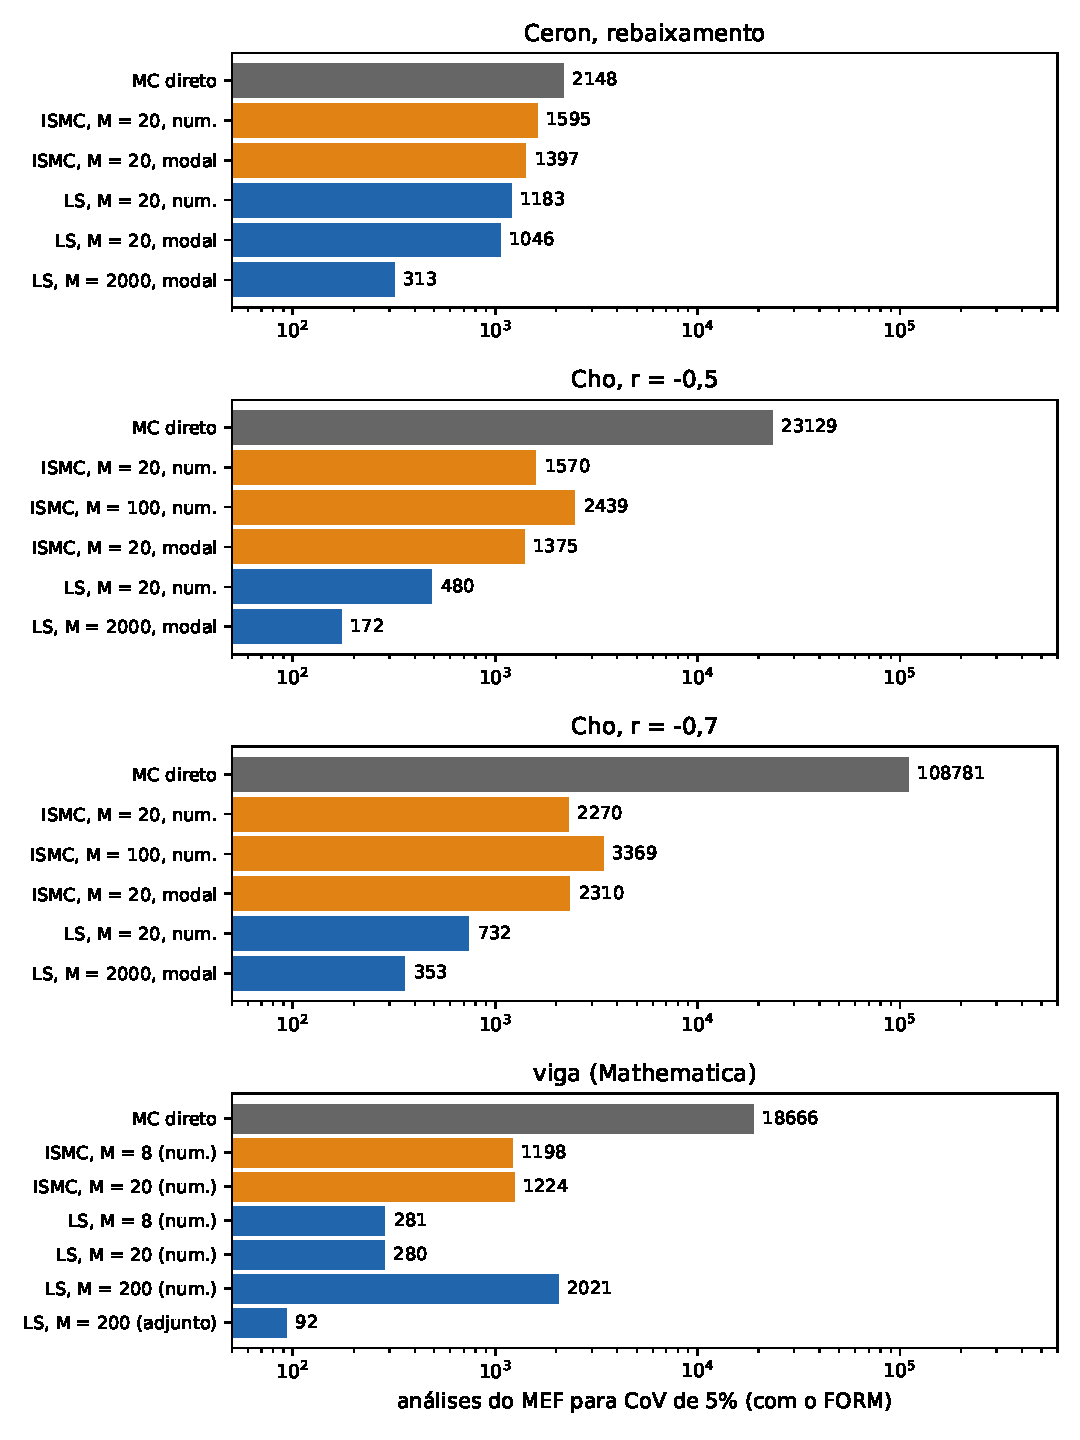
\includegraphics[width=\textwidth]{figs/custo.pdf}
\caption{Análises do MEF para CoV de 5\,\% (escala logarítmica), com o FORM. Cinza: Monte Carlo direto; laranja: ISMC;
azul: line sampling; o número ao lado de cada barra é o custo. Na viga, a direção ``adjunto'' é o FORM com o gradiente adjunto (a viga não tem gradiente modal).}\label{fig:custo}
\end{figure}

\begin{figure}[H]\centering
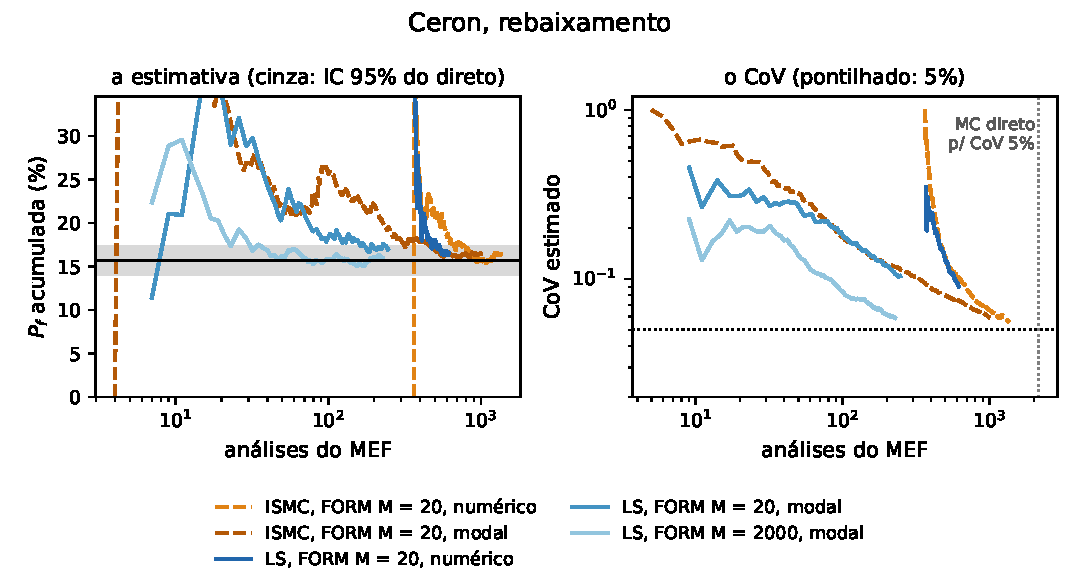
\includegraphics[width=\textwidth]{figs/convergencia_ceron.pdf}\\[2mm]
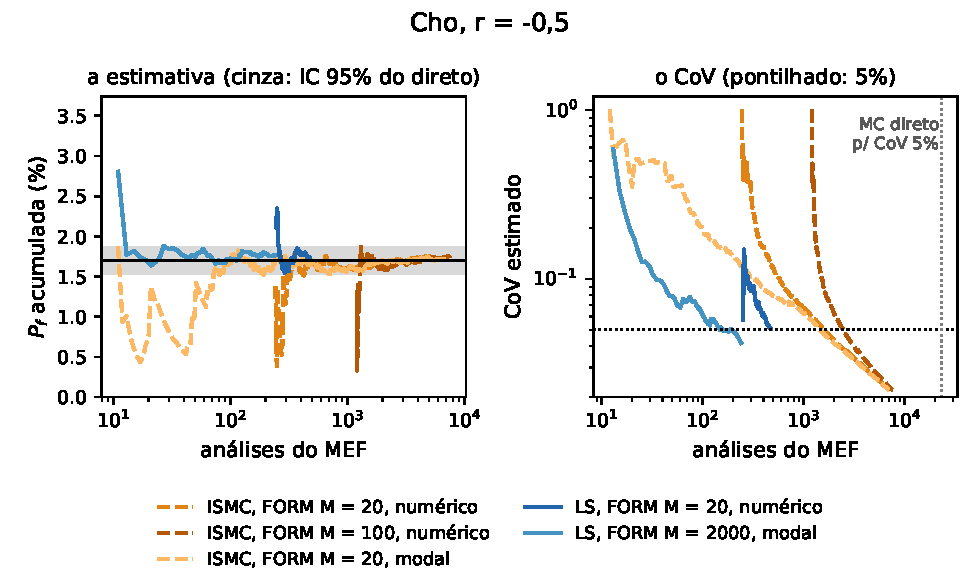
\includegraphics[width=\textwidth]{figs/convergencia_r05.pdf}
\caption{A $P_f$ acumulada (à esquerda) e o CoV estimado (à direita) contra as análises do MEF, contando o FORM (por
isso as curvas começam em pontos diferentes). Na ISMC do Cho, as 5 sementes estão em sequência. Faixa cinza: o
intervalo de 95\,\% do Monte Carlo direto; linha vertical pontilhada: o que o direto precisa para CoV de 5\,\%. O Cho com
$r = -0{,}7$ está na Figura~\ref{fig:conv2}.}\label{fig:conv}
\end{figure}
\begin{figure}[H]\centering
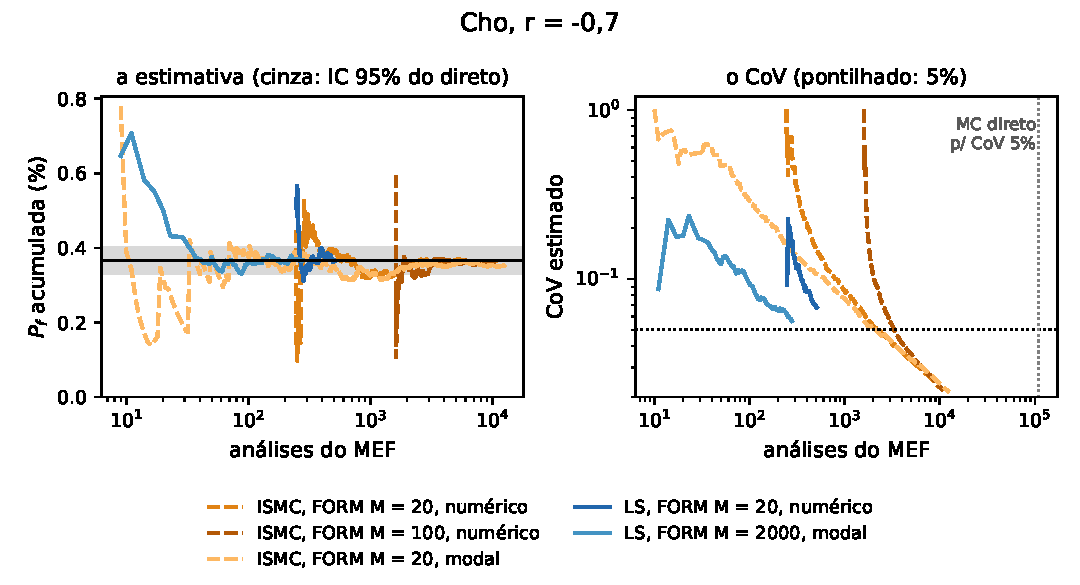
\includegraphics[width=\textwidth]{figs/convergencia_r07.pdf}
\caption{Como a Figura~\ref{fig:conv}, no Cho com $r = -0{,}7$.}\label{fig:conv2}
\end{figure}

\begin{figure}[H]\centering
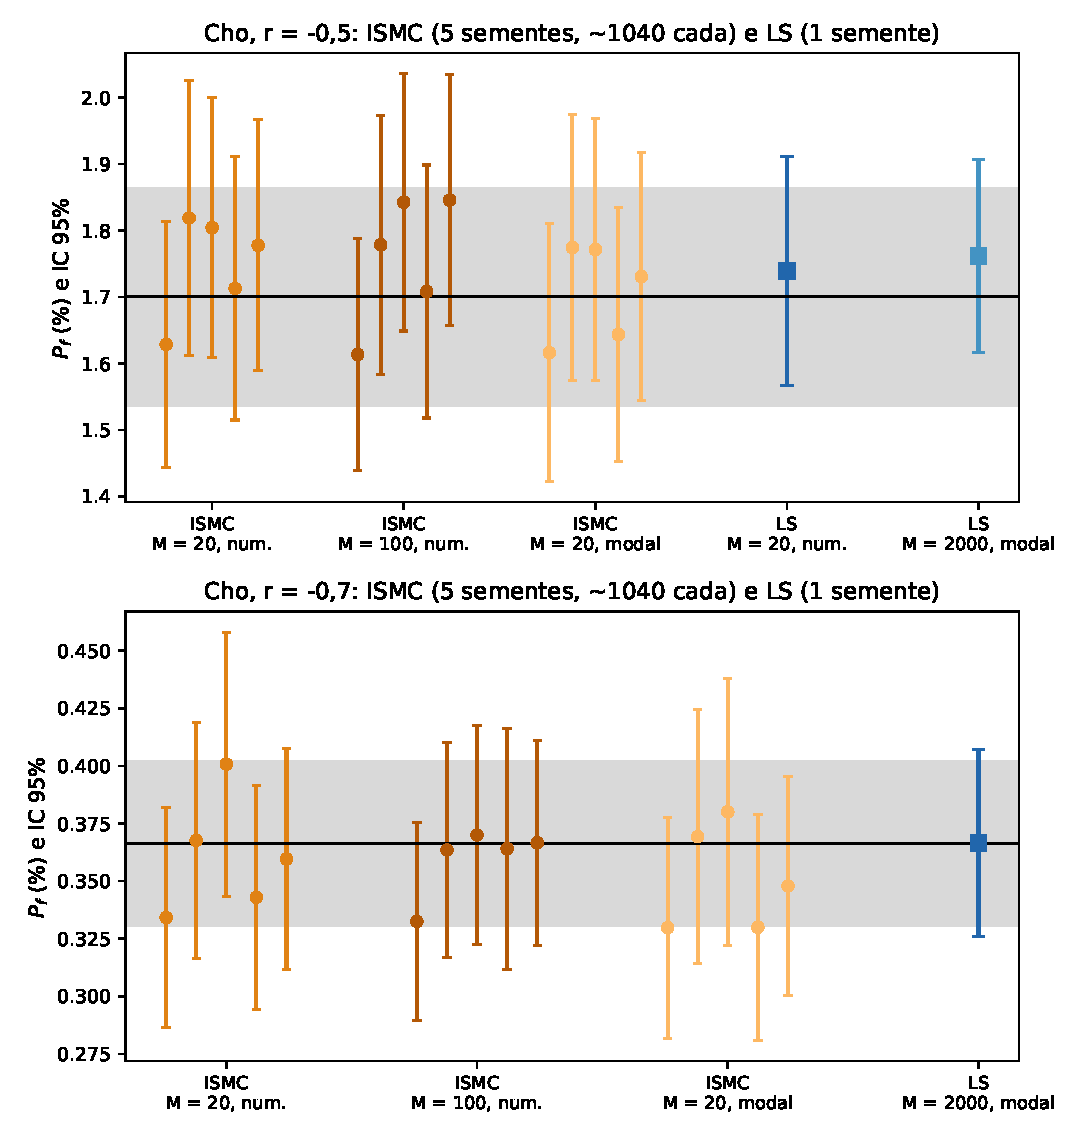
\includegraphics[width=\textwidth]{figs/sementes.pdf}
\caption{Cho: a $P_f$ de cada semente da ISMC (círculos, 5 por centro) e do line sampling (quadrados, uma semente), com
o intervalo de 95\,\% de cada uma. Faixa cinza: o intervalo do Monte Carlo direto. Todos se cruzam com o direto.}
\label{fig:sementes}
\end{figure}

\begin{figure}[H]\centering
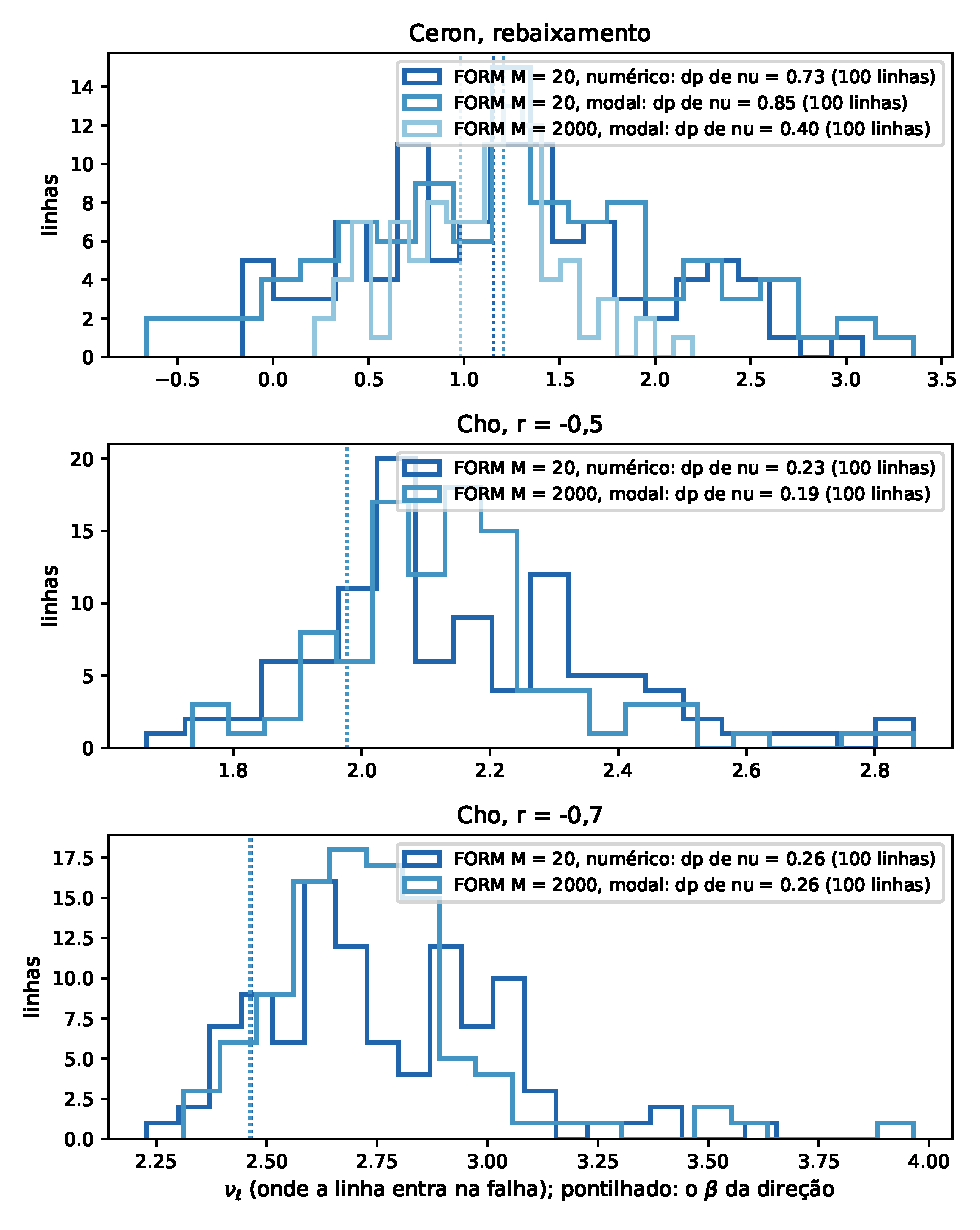
\includegraphics[width=\textwidth]{figs/linhas_nu.pdf}
\caption{Onde cada linha entra na falha ($\nu_\ell$), por direção. Uma direção que vê toda a falha dá todos os
$\nu_\ell$ perto de $\beta$ (pontilhado); a dispersão vem da curvatura e dos modos que a direção não vê. No Ceron, a
direção com 2000 termos estreita muito a distribuição.}\label{fig:nu}
\end{figure}

\section{Uma semente, pareada: SRM \texorpdfstring{$\times$}{x} GIM \texorpdfstring{$\times$}{x} análise limite}\label{sec:pareado}
Nas seções anteriores, cada método é comparado com o Monte Carlo direto, e a diferença mistura o método com o sorteio.
Aqui o que se compara é o fator de segurança: o FS do SRM, o $\Gamma$ do GIM e, quando o fermi terminar, o $\Gamma$ da
análise limite (LA: o método cinemático do Ceron 2025, \path{Projects/CeronCinematico/cho}). Os três usam as mesmas
amostras (decisão de 20/11/2026: uma semente só, pareada):
\begin{itemize}
  \item \textbf{ISMC:} a semente 21, nos três centros do FORM. A realização $n$ tem os mesmos $\xib$ e o mesmo peso $w$
    nos dois fatores: o \texttt{log\_peso} é igual em todos os pares, e as médias de $c'$ e $\varphi'$ diferem no máximo
    \sgCampo\,\% (só porque a malha adaptativa final não é a mesma no SRM e no GIM).
  \item \textbf{Line sampling:} a semente 7, as mesmas linhas (o mesmo $\bm z$ de cada uma) e as mesmas direções.
  \item \textbf{Referências:} o MC direto do SRM (24\,000 e 110\,000 realizações) e as 5 sementes da ISMC do SRM
    juntas. A conferência de versão (as 10 primeiras realizações de cada direto, refeitas com o SRM da campanha nova)
    deu o mesmo FS em \sgConfIguais{} de \sgConfTotal.
\end{itemize}
\textbf{Por que parear.} Numa semente, o erro de sorteio (o CoV de \sgCovMin{} a \sgCovMax\,\% de cada $P_f$ da
Tabela~\ref{tab:sgismc}) é o mesmo nos dois fatores, porque as realizações são as mesmas, e sai da diferença. Na ISMC,
a diferença das $P_f$ vem só dos pares em que os fatores discordam (um falha e o outro não); no line sampling, da
diferença $\Phi(-c_\text{GIM}) - \Phi(-c_\text{SRM})$ de cada linha. O seu erro é o erro pareado:
$\mathrm{dp}[w\,(I_\text{GIM} - I_\text{SRM})]/\sqrt N$ na ISMC, \sgEdifMin{} a \sgEdifMax\,\% da $P_f$ (com só
\sgDiscCasoMin{} a \sgDiscCasoMax{} pares discordantes por caso, é uma estimativa grosseira), e
$\mathrm{dp}[\Phi(-c_\text{GIM}) - \Phi(-c_\text{SRM})]/\sqrt N$ no line sampling, \sglEdifMin{} a
\sglEdifMax\,\%. Com sementes diferentes, uma diferença de 1 ou 2\,\% ficaria escondida no ruído de \sglCovMin{} a
\sgCovMax\,\% de cada estimativa.

\textbf{O GIM ainda é parcial.} Ele é a campanha \texttt{etapa3b\_gim} do fermi, que ainda roda: os dados são de
\sgData, com \sgNmin{} a \sgNmax{} realizações em comum por caso (a campanha vai a pelo menos 2000) e \sglNGmin{} a
\sglNGmax{} linhas do GIM por direção. No line sampling, entram as \sglN{} em comum com o SRM, que já estão todas
feitas: essa parte da comparação não muda mais.
% gerado por gera_dados.py (srm_gim): nao editar a mao
\begin{table}[H]\centering\footnotesize\setlength{\tabcolsep}{3pt}
\caption{A ISMC com uma semente (a 21), pareada: o SRM e o GIM nas mesmas realizações (Cho, base de Nyström de 2000 modos). \textbf{GIM parcial}: dados de 20/11/2026 18:27, com $N$ = 811 a 817 realizações em comum por caso (a campanha vai a pelo menos 2000). $P_f$ em \%: a média de $I w$ nas realizações em comum (entre parênteses, o CoV, em \%). Dif.: $(P_\text{GIM} - P_\text{SRM})/P_\text{SRM}$ $\pm$ o erro pareado, $\mathrm{dp}[w\,(I_\text{GIM} - I_\text{SRM})]/(\sqrt N\,P_\text{SRM})$. Discord.: os pares em que só o SRM falha / só o GIM falha. Referências (SRM): as 5 sementes juntas e o MC direto. LA: a análise limite na semente 21 (job 14992 do fermi, na fila).}\label{tab:sgismc}
\begin{tabular}{llrrrrcrrc}\toprule
$r$ & centro & $N$ & \makecell{SRM s21\\$P_f$ (CoV)} & \makecell{GIM s21\\$P_f$ (CoV)} & \makecell{dif.\\(\%)} & \makecell{discord.\\SRM/GIM} & \makecell{SRM\\5 sementes} & \makecell{MC\\direto} & \makecell{LA\\s21} \\\midrule
$-0{,}5$ & $M = 20$, num. & 817 & 1,617 (6,5) & 1,589 (6,6) & $-$1,7 $\pm$ 1,0 & 3/0 & 1,740 & 1,700 & rodando \\
 & $M = 100$, num. & 816 & 1,619 (6,2) & 1,579 (6,2) & $-$2,4 $\pm$ 1,4 & 3/0 & 1,745 & 1,700 & rodando \\
 & $M = 20$, modal & 815 & 1,605 (6,9) & 1,630 (6,9) & $+$1,5 $\pm$ 1,6 & 1/2 & 1,718 & 1,700 & rodando \\
\midrule
$-0{,}7$ & $M = 20$, num. & 814 & 0,3380 (8,3) & 0,3380 (8,3) & 0,0 $\pm$ 0,0 & 0/0 & 0,3656 & 0,3664 & rodando \\
 & $M = 100$, num. & 812 & 0,3417 (7,3) & 0,3371 (7,3) & $-$1,3 $\pm$ 1,3 & 1/0 & 0,3625 & 0,3664 & rodando \\
 & $M = 20$, modal & 811 & 0,3448 (8,5) & 0,3410 (8,5) & $-$1,1 $\pm$ 1,1 & 1/0 & 0,3516 & 0,3664 & rodando \\
\bottomrule\end{tabular}\end{table}


\textbf{ISMC.} Nos \sgPares{} pares (os \sgCasos{} casos juntos), só \sgDisc{} discordam: em \sgDiscSrm{} só o SRM falha
e em \sgDiscGim{} só o GIM falha (Tabela~\ref{tab:sgismc} e Figura~\ref{fig:sg}a,b). São \sgDiscDist{} realizações
distintas: com a mesma semente, a realização $n$ dos três centros de um $r$ tem a mesma amostra $\bm z$ (e
$\xib = \xib^* + \bm z$ quase igual), e algumas discordam em mais de um centro. Todos têm $|\mathrm{FS} - 1| \le$
\sgDiscFS{} e $|\Gamma - 1| \le$ \sgDiscG. Como $\Gamma \approx \mathrm{FS}^k$, com $k$ de \sgKmin{} a \sgKmax{} (perto
de 1, uma variação relativa do FS aparece \sgKperto{} vezes maior no $\Gamma$), $|\Gamma - 1| \le$ \sgDiscG{} é no
máximo \sgDiscGfs\,\% no FS. Os dois fatores só discordam a menos de \sgDiscGfs\,\% de 1, na precisão do fator (a tolerância de cada
busca e a malha adaptativa), e não por uma diferença de critério. As $P_f$ diferem de \sgDifMin{} a \sgDifMax\,\%,
sempre a menos de \sgZmax{} erros pareados; o GIM fica abaixo do SRM em \sgAbaixo{} dos \sgCasos{} casos.

\textbf{Line sampling.} Nas mesmas \sglN{} linhas, a linha do GIM entra na falha um pouco mais longe:
$\Delta c = c_\text{GIM} - c_\text{SRM}$ tem média de \sglDcMin{} a \sglDcMax{} e dp de \sglDcSdMin{} a \sglDcSdMax{}
(Tabela~\ref{tab:sgls} e Figura~\ref{fig:sg}c,d). Ao longo da linha, $d\ln\mathrm{FS}/dc$ vale $-$\sglSmin{} a
$-$\sglSmax{} (a inclinação $s$ do SRM, Tabela~\ref{tab:lsdiag}), então esse $\Delta c$ vale só uns \sglDfs\,\% no
FS (no máximo). É ele que dá a diferença das $P_f$, \sglDifMin{} a \sglDifMax\,\%: o próprio $\Delta c$ prevê \sglPrevMin{} a
\sglPrevMax\,\%, com $\Delta P_f/P_f \approx -\sum_\ell \phi(c_\ell)\,\Delta c_\ell / \sum_\ell \Phi(-c_\ell)$. Aqui o
pareamento é ainda mais forte (cada linha dá uma probabilidade contínua, e não 0 ou $w$), e a diferença, de \sglZmin{} a
\sglZmax{} erros pareados, é sistemática: o GIM dá a falha um pouquinho depois do SRM. É o mesmo sinal da ISMC
(\sgDiscSrm{} pares em que só o SRM falha, contra \sgDiscGim). Mas é pequena: \sglDifMin{} a \sglDifMax\,\% da $P_f$, contra
o CoV de \sglCovMin{} a \sglCovMax\,\% de cada estimativa.

\begin{figure}[H]\centering
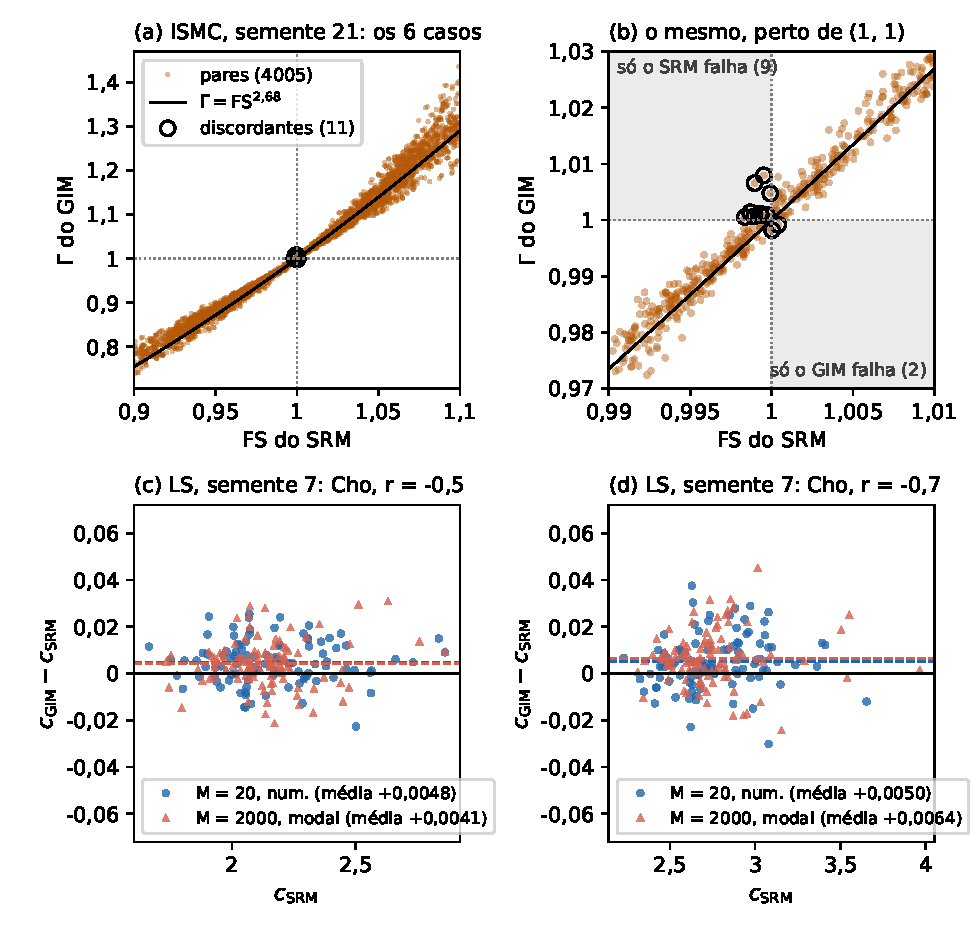
\includegraphics[width=\textwidth]{figs/srm_gim.pdf}
\caption{SRM $\times$ GIM, pareado (\textbf{GIM parcial}, dados de \sgData). (a) ISMC da semente 21: o $\Gamma$ do GIM
contra o FS do SRM na mesma realização, perto da falha ($0{,}9 < \mathrm{FS} < 1{,}1$, os seis casos juntos), com a
curva $\Gamma = \mathrm{FS}^k$ ajustada perto de 1; círculos: os pares discordantes. (b) O mesmo, perto de $(1, 1)$; em
cinza, os quadrantes em que só um dos dois falha. (c) e (d) Line sampling da semente 7: $\Delta c = c_\text{GIM} -
c_\text{SRM}$ de cada linha contra o $c_\text{SRM}$ (onde a linha do SRM entra na falha), nas \sglN{} linhas em comum de
cada direção; tracejado: a média de cada direção.}\label{fig:sg}
\end{figure}
% gerado por gera_dados.py (srm_gim): nao editar a mao
\begin{table}[H]\centering\footnotesize\setlength{\tabcolsep}{3pt}
\caption{O line sampling com uma semente (a 7), pareado: as mesmas linhas (o mesmo $\bm z$ de cada uma) e as mesmas direções, com o SRM e com o GIM. \textbf{GIM parcial}: dados de 20/11/2026 18:27; o GIM já tem 123 a 270 linhas por direção, e entram só as 100 em comum com o SRM (todas as linhas do SRM já têm o par no GIM). $P_f$ em \% (CoV em \%). Dif.: como na Tabela~\ref{tab:sgismc}, com o erro pareado das $\Phi(-c_\ell)$. $\Delta c = c_\text{GIM} - c_\text{SRM}$: onde a linha entra na falha, GIM menos SRM (média e dp das linhas). LA: o line sampling pela análise limite nas mesmas linhas (job 14992 do fermi, na fila).}\label{tab:sgls}
\begin{tabular}{llrrrrrcc}\toprule
$r$ & direção & linhas & \makecell{SRM\\$P_f$ (CoV)} & \makecell{GIM\\$P_f$ (CoV)} & \makecell{dif.\\(\%)} & \makecell{$\Delta c$\\média (dp)} & \makecell{análises por linha\\SRM / GIM} & LA \\\midrule
$-0{,}5$ & $M = 20$, num. & 100 & 1,739 (5,0) & 1,719 (5,1) & $-$1,2 $\pm$ 0,2 & $+$0,005 (0,009) & 2,31 / 2,62 & rodando \\
 & $M = 2000$, modal & 100 & 1,762 (4,2) & 1,746 (4,2) & $-$0,9 $\pm$ 0,2 & $+$0,004 (0,010) & 2,31 / 2,64 & rodando \\
\midrule
$-0{,}7$ & $M = 20$, num. & 100 & 0,3642 (6,8) & 0,3605 (6,9) & $-$1,0 $\pm$ 0,3 & $+$0,005 (0,011) & 2,64 / 2,92 & rodando \\
 & $M = 2000$, modal & 100 & 0,3665 (5,6) & 0,3603 (5,7) & $-$1,7 $\pm$ 0,3 & $+$0,006 (0,012) & 2,72 / 2,97 & rodando \\
\bottomrule\end{tabular}\end{table}


\textbf{Conclusão.}
\begin{itemize}
  \item \textbf{O GIM e o SRM dão a mesma $P_f$ a menos de \sgDifAbsMax\,\%} (com a ISMC do GIM parcial): na ISMC,
    \sgDifMin{} a \sgDifMax\,\%, dentro do ruído pareado, e a diferença vem só das realizações limítrofes
    ($|\mathrm{FS} - 1| \le$ \sgDiscFS); no line sampling, mais preciso, \sglDifMin{} a \sglDifMax\,\%, de um
    deslocamento de \sglDcMin{} a \sglDcMax{} em $c$ (uns \sglDfs\,\% no FS). O GIM fica um pouco abaixo (de forma
    sistemática no line sampling), mas bem dentro do CoV de cada estimativa: para a confiabilidade, os dois fatores dão
    a mesma resposta.
  \item \textbf{A semente 21 é baixa em $r = -0{,}5$.} Das 5 sementes do SRM, ela é a mais baixa nos três centros:
    \sUmRaMin{} a \sUmRaMax\,\% com todas as suas realizações, contra \sOutRaMin{} a \sOutRaMax\,\% das outras quatro,
    \sJunRaMin{} a \sJunRaMax\,\% das 5 juntas e \refPfRa{} do direto (Tabela~\ref{tab:ismcsem}). Por isso o SRM e o
    GIM da semente 21 ficam abaixo do direto: é a semente, e não o método. Em $r = -0{,}7$ ela fica no meio das 5
    (posições \sPosRb{} nos três centros: \sUmRbMin{} a \sUmRbMax\,\%, contra \sJunRbMin{} a \sJunRbMax\,\% das 5
    juntas). Na Tabela~\ref{tab:sgismc}, porém, entram só as realizações em comum, as primeiras da semente: nelas, o
    SRM e o GIM dão \sgSubRaMin{} a \sgSubRaMax\,\% com $r = -0{,}5$ e \sgSubRbMin{} a \sgSubRbMax\,\% com
    $r = -0{,}7$, abaixo da semente inteira em todos os centros. É o sorteio dessas realizações (CoV de \sgCovMin{} a
    \sgCovMax\,\%), igual nos dois fatores, e muda quando o GIM chegar ao fim.
  \item \textbf{Custo.} Nas mesmas realizações, uma análise do GIM leva \sgTgimMin{} a \sgTgimMax\,s no fermi, contra
    \sgTsrmMin{} a \sgTsrmMax\,s do SRM: \sgEcon\,\% menos. No line sampling, o GIM gastou um pouco mais por linha
    (\sglNaGimMin{} a \sglNaGimMax{} análises, contra \sglNaSrmMin{} a \sglNaSrmMax{} do SRM), e o custo por linha
    quase empata (\sglCustoMin{} a \sglCustoMax\,\% para o GIM, com o custo por análise da ISMC). O ganho grande está
    no FORM modal, que usa o gradiente do GIM: \fgNRa{} análises com $r = -0{,}5$ e \fgNRb{} com $r = -0{,}7$ (2000
    modos por campo; $\beta$ = \fgBetaRa{} e \fgBetaRb), contra as \fnNRa{} do FORM numérico com $M = 20$ ($\beta$ =
    \fnBetaRa{} e \fnBetaRb).
  \item \textbf{Análise limite: rodando no fermi} desde 20/11/2026 às 18:06. O job 14991 faz o MC direto com
    $r = -0{,}5$ e $-0{,}7$, pareado realização a realização com o direto do SRM (e com $r = 0$, para conferir com o
    Ceron); às \laLogHora, tinha \laLogN{} realizações de $r$ = \laLogR. O job 14992 (o FORM, o line sampling da semente
    7 e a ISMC da semente 21) espera vaga. A coluna ``LA'' das Tabelas~\ref{tab:sgismc} e \ref{tab:sgls} fica para
    quando terminar. No piloto local (\path{Projects/CeronCinematico/cho/resultados/piloto_h0.025}: \laN{} realizações
    do direto de cada $r$, grade de $h = 0{,}025$\,m), $\mathrm{FS}_\text{LA} - \mathrm{FS}_\text{MEF}$ = \laDif{} em
    média (+\laRelMin{} e +\laRelMax\,\% nos dois $r$; de +\laRelLo{} a +\laRelHi\,\% por realização), com
    correlação de \laCorr, e $\mathrm{FS}_\text{LA} > \mathrm{FS}_\text{MEF}$ em \laAcima{} das \laTotal{} realizações:
    a análise limite, um limite superior com bloco rígido, fica uns 3\,\% acima do MEF, e espera-se
    $P_f(\text{LA}) < P_f(\text{MEF})$ (no piloto, \laFalLa{} falhas na LA e \laFalMef{} no MEF, nas mesmas
    \laTotal{} realizações).
\end{itemize}

\section{O Ceron com a água do artigo}\label{sec:ceronagua}
As linhas do Ceron nas outras seções (Tabelas~\ref{tab:ref}, \ref{tab:form} e \ref{tab:ceron}, as seguintes e as
figuras) usam o \textbf{modelo de água antigo}: o rebaixamento em 0,1\,h, com o transiente da água não saturada e
os nossos contornos do reservatório (\texttt{trebaix=0.1 agua=unsat contorno=reservatorio}), e o GIM com 3 níveis de
refinamento ($\Gamma$ determinístico de \ceaGvelho; $P_f$ do direto de \refPfCe). A comparação dos métodos continua
valendo, porque o problema é o mesmo para todos eles, mas essa $P_f$ não é a do artigo (\ceaPfArt). Com a \textbf{água
do artigo} (o solo saturado, o rebaixamento instantâneo e os contornos das Eqs.~19--21 do Ceron, de pressão imposta,
sem face de percolação e com a lateral direita sem fluxo: \texttt{agua=sat trebaix=0.0001 contorno=ceron}; com a água
saturada, praticamente sem armazenamento, o fluxo é o de Darcy permanente) e 5 níveis (Tabela~\ref{tab:ceronagua}):
\begin{itemize}
  \item \textbf{O determinístico:} o $\Gamma$ do GIM extrapolado dos níveis 3, 4 e 5 (\ceaGniveis) é \ceaGdetPz,
    contra \ceaGdetArt{} do artigo e \ceaGdetLa{} da nossa análise limite em Python.
  \item \textbf{O line sampling do MEF} (o GIM, na direção do FORM modal com 2000 termos: \ceaForm{} análises,
    $\beta$ = \ceaBeta) parou com CoV de 5\,\% em \ceaLsN{} linhas (\ceaLsAn{} análises): $P_f$ = \ceaLsPf{} (IC de
    95\,\%: \ceaLsLo{} a \ceaLsHi), contra \ceaPfArt{} do artigo ($z$ = \ceaLsZ).
  \item \textbf{O MC de \ceaMcN{} realizações pela análise limite em Python} (a configuração de referência do artigo):
    \ceaMcPf{} com a busca rápida. Refeitas com a busca exata as \ceaMcRef{} realizações com
    $1{,}0 \le \Gamma < 1{,}10$, aparecem \ceaMcNovas{} falhas novas, e a $P_f$ vai a \ceaMcPfEx{} ($\pm$ \ceaMcIc,
    95\,\%). A média de $\Gamma$ é \ceaGmedLa{} (artigo: \ceaGmedArt, do ajuste lognormal).
\end{itemize}
% gerado por gera_dados.py (ceron_agua): nao editar a mao
\begin{table}[H]\centering\footnotesize\setlength{\tabcolsep}{4pt}
\caption{O rebaixamento do Ceron com a água do artigo (\texttt{agua=sat trebaix=0.0001 contorno=ceron}). IC de 95\,\%: $P_f(1 \pm 1{,}96\,\mathrm{CoV})$ (no artigo, com o CoV de 2,77\,\% que ele dá). $z$: a diferença contra o artigo, em desvios padrão. $\Gamma$ det.: o determinístico (as médias de $c'$, $\varphi'$ e $k$); $^*$: extrapolado dos níveis 3 a 5 do GIM (1,401; 1,366; 1,351). Na última linha, a referência das outras seções, com a água antiga.}\label{tab:ceronagua}
\begin{tabular}{lrrrrr}\toprule
método e amostra & $P_f$ & IC de 95\,\% & $z$ & $\Gamma$ det. & média de $\Gamma$ \\\midrule
Ceron (2025): análise limite, MC de 10\,000 & 11,50\,\% & 10,88--12,12\,\% & -- & 1,336 & 1,353 \\
MEF (GIM, 5 níveis): LS, 153 linhas e 4 + 363 análises & 11,61\,\% & 10,49--12,73\,\% & $+$0,2 & 1,340$^*$ & -- \\
análise limite (Python): MC de 10\,000, busca rápida & 10,29\,\% & 9,69--10,89\,\% & $-$2,7 & 1,347 & 1,384 \\
\quad e a busca exata nas 993 com $1 \le \Gamma < 1{,}1$ & 10,32\,\% & 9,72--10,92\,\% & $-$2,7 &  & 1,384 \\
\midrule
MEF (GIM, 3 níveis): MC direto de 2\,000, água antiga & 15,70\,\% & 14,11--17,29\,\% & $+$4,8 & 1,325 & 1,294 \\
\bottomrule\end{tabular}\end{table}

O MEF com a água do artigo reproduz a $P_f$ do artigo: \ceaLsPf{} contra \ceaPfArt, a \ceaLsDifPt{} ponto, dentro do
IC. A nossa análise limite fica \ceaMcDifPt{} ponto abaixo do artigo, fora do IC ($z$ = \ceaMcZ), e a média de $\Gamma$
fica acima (\ceaGmedLa{} contra \ceaGmedArt): essa diferença para o MC do artigo ainda não está explicada. A busca
rápida não a explica: a busca exata mudou $\Gamma$ em mais de 1\,\% em só \ceaExMuda{} das \ceaMcRef{} realizações
refeitas (no máximo \ceaExMax\,\%), e a $P_f$ subiu \ceaMcSobe{} ponto. Que a nossa análise limite dê uma $P_f$ abaixo
da do MEF tem o sinal de um limite superior, mas isso não explica a diferença toda: no determinístico, os dois quase
coincidem ($\Gamma$ = \ceaGdetLa{} na análise limite, contra \ceaGdetPz{} do MEF extrapolado e \ceaGnivelFim{} com os 5
níveis que o line sampling usa), e a análise limite do artigo dá a mesma $P_f$ do nosso MEF. A diferença para a
referência antiga (\refPfCe) é a água (e a malha: 3 níveis lá, 5 aqui).

\section{Tempo de CPU}\label{sec:tempo}
Todos os processos rodam com uma \emph{thread} (\texttt{PZ\_THREADS=0}, OpenMP e MKL com 1), então o tempo de
uma análise gravado no CSV (\texttt{s\_fator}, mais \texttt{s\_transiente} no Ceron) é a CPU dela. A
Tabela~\ref{tab:tempo} soma esses tempos por método; o custo para CoV de 5\,\% em h$\cdot$núcleo é o número de análises
da Tabela~\ref{tab:ceron}--\ref{tab:r07} vezes o custo unitário da última coluna, mais o FORM.
\begin{itemize}
  \item \textbf{Cho (fermi):} uma análise do SRM custa \uDirRa{}\,s no direto com $r = -0{,}5$ e \uDirRb{}\,s com
    $r = -0{,}7$, e \uAmRa{} e \uAmRb{}\,s nas ISMC (base de Nyström). Os dois diretos gastaram \hDirTotalCho{}
    h$\cdot$núcleo; as 30 ISMC da etapa 3b, \hIsmcTotal{} (\hIsmcBlocos{} h somando a parede dos blocos: ler a malha e
    gravar custam uns 3\,\%). Para CoV de 5\,\%: com $r = -0{,}5$, \hDirRa{}~h no direto, \hIsmcRa{}~h na melhor ISMC e
    \hLsRa{}~h no line sampling modal; com $r = -0{,}7$, \hDirRb{}, \hIsmcRb{} e \hLsRb{}~h.
  \item \textbf{Line sampling:} o \texttt{line\_sampling.py} apaga os CSV de cada análise, então não há tempo por
    análise. A estimativa usa o custo unitário das ISMC do mesmo $r$ (o mesmo SRM, a mesma malha, no fermi). A parede no
    PC vezes os processos é só um teto (há núcleos ociosos no fim, e o PC é outra máquina).
  \item \textbf{Ceron (PC, 8 núcleos físicos):} o direto rodou com 8 processos (\uDirCe{}\,s por análise); a ISMC e o
    FORM numérico, com 13 ou 14 (54\,s por análise). A mesma análise do campo médio (a realização $-1$) levou 34\,s no
    direto e 65\,s na ISMC, então a diferença é do PC, não do método: provavelmente a disputa de núcleo (14 processos em 8
    núcleos físicos; o executável do direto também era outra cópia). Para comparar os métodos, todos usam o custo do
    direto, \uDirCe{}\,s, inclusive o FORM numérico (363 análises $\times$ \uDirCe{}\,s; a CPU medida foi de
    \formCeronCpu{}\,h); as horas medidas da amostragem estão na tabela só como informação.
  \item \textbf{FORM modal:} cada análise do GIM é mais barata que a do SRM (\gimCpuIt{}\,s no PC e
    \gimCpuItFermi{}\,s no fermi, contra uns 65\,s do SRM no fermi), mas a parede de uma iteração com 2000 modos no PC
    foi de \gimParedeIt{} min: gerar o campo e projetar o gradiente modal
    custam mais que a própria análise. Por isso o custo do FORM modal na tabela é a parede, não a CPU das análises.
    Mesmo assim, o FORM modal custa 0,06 a 0,2 h, contra 4 h do numérico com $M = 20$ e 20 a 26 h com $M = 100$ (Cho).
  \item \textbf{Viga:} uma análise leva uns 8\,ms (Mathematica); os tempos são de parede, com os \emph{kernels} em
    paralelo, e o número de \emph{kernels} não foi gravado. Na viga, a comparação é só pelo número de análises.
\end{itemize}
% gerado por gera_dados.py: nao editar a mao
\begin{landscape}
\begin{table}[H]\centering\footnotesize
\caption{O tempo de CPU (h$\cdot$núcleo; cada processo roda com 1 \emph{thread}, então a CPU de uma análise é o seu tempo de parede). ``s/análise'': a média medida (\texttt{s\_fator}, mais \texttt{s\_transiente} no Ceron). FORM: numérico, CPU somada das análises; modal, a parede (em série; inclui o campo e o gradiente modal). No Ceron (PC), o FORM numérico e as colunas ``p/ CoV 5\,\%'' usam as análises $\times$ o custo unitário do direto, \uDirCe{}\,s (a CPU medida do FORM numérico, \formCeronCpu{}\,h, inflada pela disputa de núcleo, está na Tabela~\ref{tab:formit}); ``s/análise'' e ``amostragem'' são as medidas. Amostragem: o que já foi gasto. ``Parede dos blocos'': a soma dos tempos dos blocos nos logs do fermi (inclui ler a malha e gravar). LS: sem tempo por análise; a estimativa usa o custo unitário da última coluna, e a parede do PC $\times$ processos é um teto. ``p/ CoV 5\,\%'': o FORM mais as análises para CoV de 5\,\% vezes o custo unitário.}\label{tab:tempo}
\begin{tabular}{llrrrrrrr}\toprule
problema & método e centro/direção & \makecell{s/análise\\medido} & \makecell{FORM\\(h)} & \makecell{amostragem\\(h)} & \makecell{parede dos\\blocos (h)} & \makecell{PC: parede\\$\times$ proc. (h)} & \makecell{p/ CoV\\5\,\% (h)} & \makecell{custo\\unitário (s)} \\\midrule
Ceron, rebaixamento & MC direto (2\,000) & 35,6 & -- & 19,8 & -- & -- & 21,3 & 35,6 \\
 & ISMC, $M = 20$, num. & 54,3 & 3,59 & 15,1 & -- & -- & 15,8 & 35,6 \\
 & ISMC, $M = 20$, modal & 54,8 & 0,06 & 15,2 & -- & -- & 13,9 & 35,6 \\
 & LS, $M = 20$, num. & -- & 3,59 & $\approx$2,5 & -- & 4,5 (14) & 11,7 & 35,6 \\
 & LS, $M = 20$, modal & -- & 0,06 & $\approx$2,4 & -- & 4,1 (14) & 10,4 & 35,6 \\
 & LS, $M = 2000$, modal & -- & 0,06 & $\approx$2,2 & -- & 3,9 (14) & 3,1 & 35,6 \\
\midrule
Cho, $r = -0{,}5$ & MC direto (24\,000) & 69,2 & -- & 461,4 & 463,8 & -- & 444,7 & 69,2 \\
 & ISMC, $M = 20$, num. & 65,9 & 4,04 & 123,5 & 127,2 & -- & 28,3 & 65,9 \\
 & ISMC, $M = 100$, num. & 65,6 & 19,73 & 114,2 & 117,6 & -- & 42,2 & 65,6 \\
 & ISMC, $M = 20$, modal & 66,0 & 0,11 & 128,4 & 132,1 & -- & 25,1 & 66,0 \\
 & LS, $M = 20$, num. & -- & 4,04 & $\approx$4,3 & -- & 5,1 (14) & 8,4 & 65,8 \\
 & LS, $M = 2000$, modal & -- & 0,21 & $\approx$4,3 & -- & 5,2 (14) & 3,2 & 65,8 \\
\midrule
Cho, $r = -0{,}7$ & MC direto (110\,000) & 68,2 & -- & 2\,084,6 & 2\,095,4 & -- & 2\,061,5 & 68,2 \\
 & ISMC, $M = 20$, num. & 63,4 & 3,96 & 185,3 & 191,0 & -- & 39,7 & 63,4 \\
 & ISMC, $M = 100$, num. & 63,0 & 26,20 & 159,1 & 164,0 & -- & 57,1 & 63,0 \\
 & ISMC, $M = 20$, modal & 64,2 & 0,09 & 222,7 & 229,4 & -- & 41,1 & 64,2 \\
 & LS, $M = 20$, num. & -- & 3,96 & $\approx$4,7 & -- & 5,7 (14) & 12,6 & 63,6 \\
 & LS, $M = 2000$, modal & -- & 0,14 & $\approx$4,8 & -- & 5,2 (12) & 6,3 & 63,6 \\
\bottomrule\end{tabular}\end{table}
\end{landscape}


\section{As iterações do FORM}\label{sec:form}
A Tabela~\ref{tab:formit} e a Figura~\ref{fig:formit} mostram o histórico de cada FORM (o \texttt{historico} do
\texttt{form.json}). O FORM numérico (SRM) convergiu em 3 iterações (4 no $M = 100$ com $r = -0{,}7$), com
$4M + 1$ análises por iteração. O FORM modal usa o GIM, em que $g = \Gamma - 1$ começa em 0,616 (no SRM, $g = \mathrm{FS} - 1$
começa em 0,168): a escala é outra, e por isso a figura usa $|g/g_0|$. No Cho, o modal precisou de 5 a 10 iterações:
$\beta$ chega ao valor final em 3 ou 4, mas $\Gamma$ oscila uns $\pm 0{,}003$ entre análises vizinhas (o ruído do
refinamento adaptativo), e o critério $|g| < 10^{-3}$ só é atendido depois de algumas voltas. Como cada iteração custa
uma análise, isso pouco pesa. No Ceron, os três FORM convergiram em 3 iterações. Na viga só o número de análises foi
gravado; as 4 iterações saem da contagem, $1 + 4(2M + 1) + 2M$.
% gerado por gera_dados.py
\begin{table}[H]\centering\footnotesize\setlength{\tabcolsep}{3pt}
\caption{Os FORM, iteração a iteração resumidos: iterações, análises, $g$ inicial e final ($\mathrm{FS} - 1$ no SRM, $\Gamma - 1$ no GIM), $\beta$, a CPU das análises e a parede (do primeiro arquivo de parâmetros ao \texttt{form.json}). $\alpha^2$: a parte da variância linearizada em cada campo.}\label{tab:formit}
\begin{tabular}{llrrrrrrrl}\toprule
problema & FORM & it. & análises & $g_0$ & $g$ final & $\beta$ & \makecell{CPU\\(h)} & \makecell{parede\\(h)} & \makecell{$\alpha^2$\\($c'$, $\varphi'$, $k$)} \\\midrule
Ceron, rebaixamento & $M = 20$, num. (GIM) & 3 & 363 & 0,241 & 0,0001 & 1,153 & 5,39 & 0,45 & 0,83, 0,09, 0,08 \\
 & $M = 20$, modal (GIM) & 3 & 3 & 0,241 & -0,0002 & 1,205 & 0,05 & 0,06 & 0,89, 0,11, 0,00 \\
 & $M = 2000$, modal (GIM) & 3 & 3 & 0,241 & 0,0003 & 0,982 & 0,06 & 0,06 & 0,88, 0,12, 0,00 \\
Cho, $r = -0{,}5$ & $M = 20$, num. (SRM) & 3 & 243 & 0,168 & 0,0008 & 1,977 & 4,04 & 0,36 & 0,06, 0,94 \\
 & $M = 100$, num. (SRM) & 3 & 1203 & 0,168 & 0,0009 & 1,956 & 19,73 & 1,70 & 0,07, 0,93 \\
 & $M = 20$, modal (GIM) & 10 & 10 & 0,616 & 0,0008 & 2,003 & 0,10 & 0,11 & 0,05, 0,95 \\
 & $M = 2000$, modal (GIM) & 7 & 7 & 0,616 & 0,0004 & 1,977 & 0,05 & 0,21 & 0,05, 0,95, 0,00 \\
Cho, $r = -0{,}7$ & $M = 20$, num. (SRM) & 3 & 243 & 0,168 & 0,0007 & 2,466 & 3,96 & 0,35 & 0,03, 0,97 \\
 & $M = 100$, num. (SRM) & 4 & 1604 & 0,168 & 0,0005 & 2,440 & 26,20 & 2,25 & 0,03, 0,97 \\
 & $M = 20$, modal (GIM) & 8 & 8 & 0,616 & 0,0008 & 2,492 & 0,08 & 0,09 & 0,02, 0,98 \\
 & $M = 2000$, modal (GIM) & 5 & 5 & 0,616 & 0,0007 & 2,463 & 0,03 & 0,14 & 0,02, 0,98, 0,00 \\
viga & $M = 8$, num. & 4 & 85 & -- & -- & 2,149 & \multicolumn{2}{c}{1,6 s (parede)} & -- \\
 & $M = 20$, num. & 4 & 205 & -- & -- & 2,130 & \multicolumn{2}{c}{2,7 s (parede)} & -- \\
 & $M = 200$, num. & 4 & 2005 & -- & -- & 2,118 & \multicolumn{2}{c}{16,3 s (parede)} & -- \\
 & $M = 200$, adjunto & 4 & 15 & -- & -- & 2,130 & \multicolumn{2}{c}{5,4 s (parede)} & -- \\
\bottomrule\end{tabular}\end{table}

\begin{figure}[H]\centering
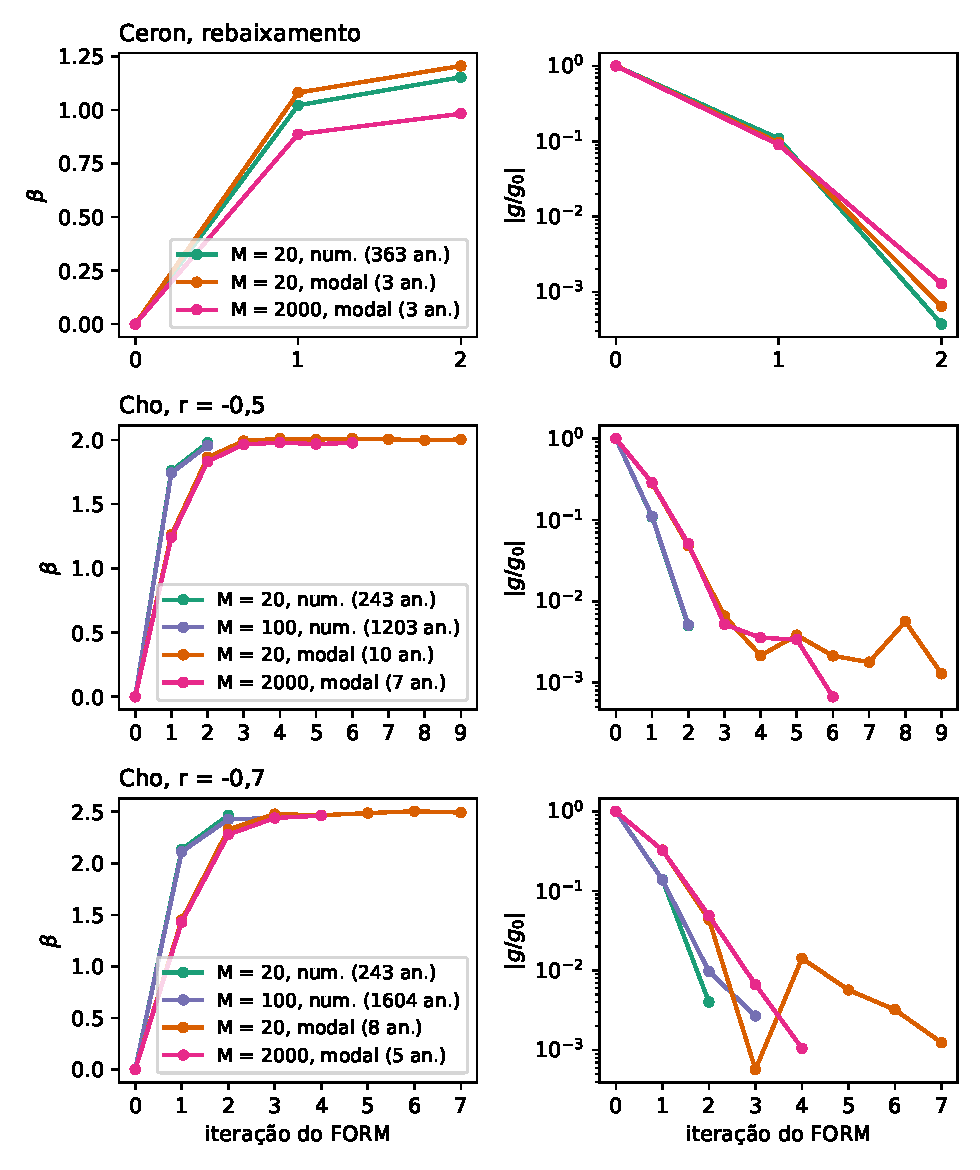
\includegraphics[width=\textwidth]{figs/form_iteracoes.pdf}
\caption{O FORM iteração a iteração: $\beta$ (à esquerda) e $|g/g_0|$ (à direita, escala logarítmica). Na legenda,
as análises de cada FORM.}\label{fig:formit}
\end{figure}

\section{Convergência e eficiência}\label{sec:efic}
Em todos os métodos, o CoV cai como $1/\sqrt{n}$, em que $n$ é o número de análises da amostragem (amostras ou
análises das linhas). Então $\delta_1 = \mathrm{CoV}\sqrt{n}$, o CoV que uma análise sozinha daria, resume o método: para
CoV de 5\,\% são $(\delta_1/0{,}05)^2$ análises, mais o FORM. As Figuras~\ref{fig:eficCe}--\ref{fig:eficViga} mostram
o CoV contra $n$ em escala log-log, com as retas $\delta_1/\sqrt{n}$ (pontilhadas), e o $\delta_1$ corrente, que fica
constante quando a variância já está bem estimada. No direto, $\delta_1 = \sqrt{(1 - P_f)/P_f}$: 2,3 no Ceron,
7,6 e 16,5 no Cho. Nas ISMC do Cho, $\delta_1 \approx 1{,}8$ a 2,4; no line sampling do Cho, 0,6 a 1,1.

A figura de mérito usual é $1/(\mathrm{CoV}^2 \times \text{custo})$, e a eficiência relativa é a figura de mérito do método
dividida pela do direto (Tabela~\ref{tab:efic} e Figura~\ref{fig:eficbar}). Ela tem três versões:
\begin{itemize}
  \item \textbf{por análise de amostragem}, $(\delta_{1,\text{dir}}/\delta_1)^2$, sem contar o FORM. É o que o método
    faz com cada análise: até \efAIsmcRb{} vezes o direto na ISMC e \efALsRb{} no line sampling (Cho, $r = -0{,}7$);
  \item \textbf{com o FORM, em análises}, a razão das análises para CoV de 5\,\% (o ``ganho'' das
    Tabelas~\ref{tab:ceron}--\ref{tab:r07});
  \item \textbf{com o FORM, em h$\cdot$núcleo}: no line sampling modal, \efHLsCe, \efHLsRa{} e \efHLsRb{} vezes o direto
    no Ceron e no Cho. Fica perto da versão em análises, porque o FORM modal é barato e o custo de uma análise quase não
    muda entre os métodos.
\end{itemize}
A diferença entre a primeira e a segunda versão é o preço do FORM. Ela é grande no FORM numérico com muitos termos: na
viga, o line sampling com a direção do FORM numérico $M = 200$ tem o melhor $\delta_1$ de todos (0,19), mas as 2005
análises do FORM derrubam a eficiência total para 9 vezes o direto; a direção do FORM adjunto, quase tão boa e com 15
análises, chega a 200 vezes.

\begin{figure}[H]\centering
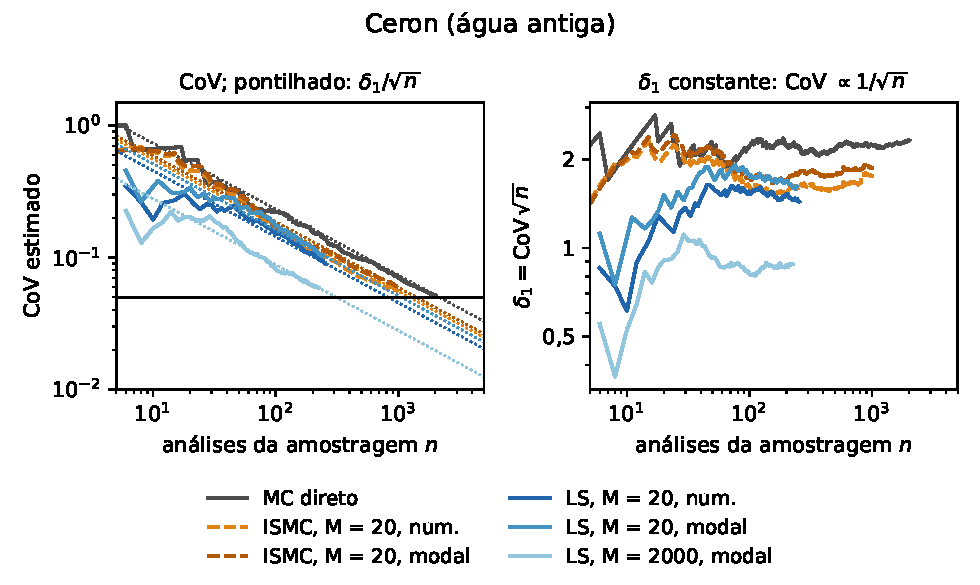
\includegraphics[width=\textwidth]{figs/eficiencia_ceron.pdf}\\[2mm]
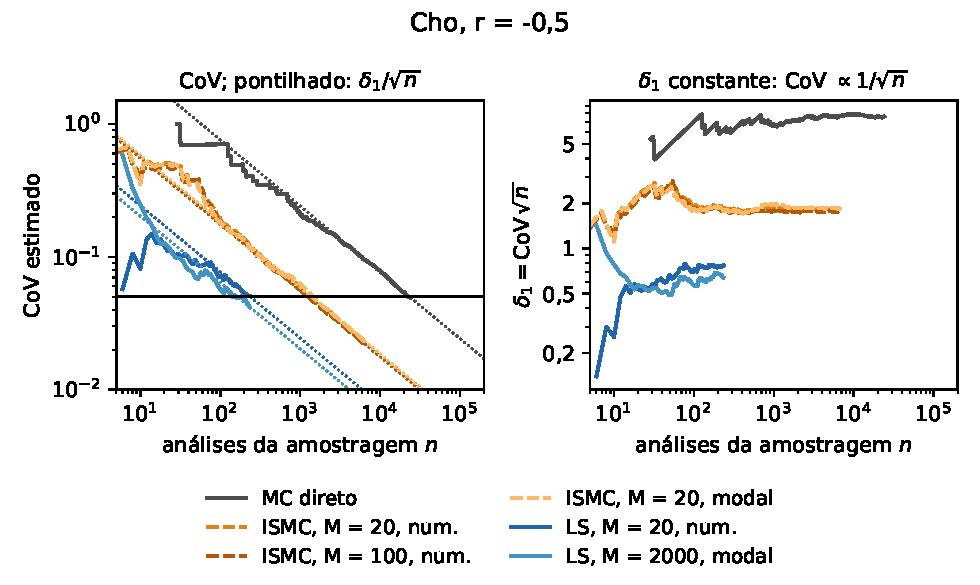
\includegraphics[width=\textwidth]{figs/eficiencia_r05.pdf}
\caption{Ceron e Cho com $r = -0{,}5$. À esquerda, o CoV estimado contra as análises da amostragem $n$ (sem o FORM),
em log-log; pontilhado, a reta $\delta_1/\sqrt{n}$ com o $\delta_1$ final de cada método; linha cheia, CoV de 5\,\%.
À direita, $\delta_1 = \mathrm{CoV}\sqrt{n}$ corrente: quanto mais baixo, mais eficiente o método por análise. Na ISMC do
Cho, as 5 sementes em sequência.}\label{fig:eficCe}
\end{figure}
\begin{figure}[H]\centering
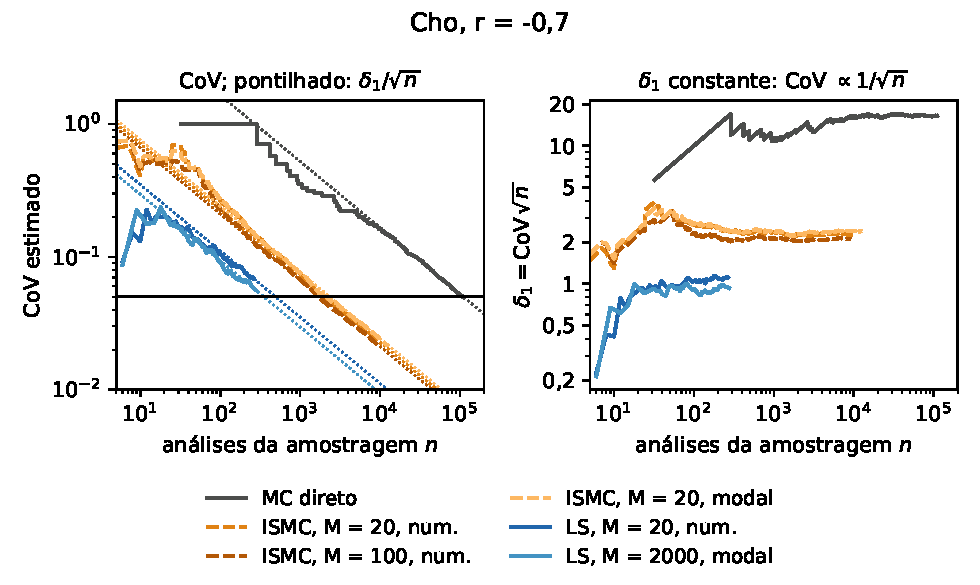
\includegraphics[width=\textwidth]{figs/eficiencia_r07.pdf}\\[2mm]
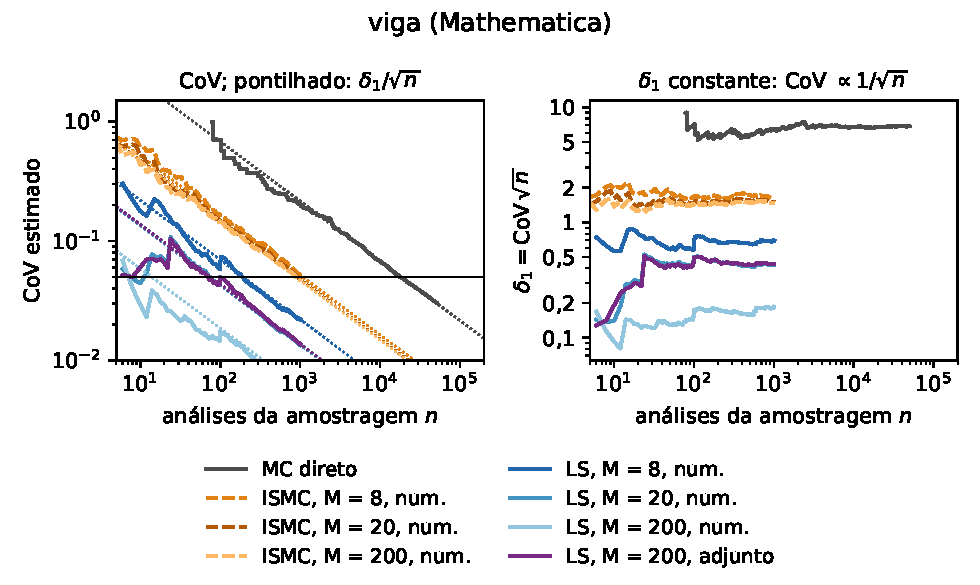
\includegraphics[width=\textwidth]{figs/eficiencia_viga.pdf}
\caption{Como a Figura~\ref{fig:eficCe}, no Cho com $r = -0{,}7$ e na viga (direto de 50\,000, ISMC de 1000 com uma
semente e line sampling de 500 linhas).}\label{fig:eficViga}
\end{figure}
% gerado por gera_dados.py
\begin{landscape}
\begin{table}[H]\centering\footnotesize
\caption{A eficiência. $\delta_1 = \mathrm{CoV}\sqrt{n}$: o CoV de uma análise de amostragem ($n$: as análises da amostragem, sem o FORM); no direto, $\sqrt{(1 - P_f)/P_f}$. Com $\mathrm{CoV} = \delta_1/\sqrt{n}$, o $n$ para CoV de 5\,\% é $(\delta_1/0{,}05)^2$. Figura de mérito: $1/(\mathrm{CoV}^2 \times \text{custo})$; a eficiência relativa é a figura de mérito do método dividida pela do direto: por análise de amostragem, $(\delta_{1,\text{dir}}/\delta_1)^2$; com o FORM, a razão das análises para CoV de 5\,\% (o ``ganho'' das tabelas anteriores); em tempo, a razão das h$\cdot$núcleo para CoV de 5\,\% (Tabela~\ref{tab:tempo}).}\label{tab:efic}
\begin{tabular}{lllrrrrrr}\toprule
problema & método & centro ou direção & $n$ & CoV & $\delta_1$ & efic. por análise & efic. com o FORM & efic. em tempo \\\midrule
Ceron (água antiga) & MC direto & -- & 2\,000 & 5,2\,\% & 2,32 & 1,0× & 1,0× & 1,0× \\
 & ISMC & $M = 20$, num. & 1\,000 & 5,6\,\% & 1,76 & 1,7× & 1,3× & 1,3× \\
 & ISMC & $M = 20$, modal & 1\,000 & 5,9\,\% & 1,87 & 1,5× & 1,5× & 1,5× \\
 & LS (100 lin.) & $M = 20$, num. & 254 & 9,0\,\% & 1,44 & 2,6× & 1,8× & 1,8× \\
 & LS (100 lin.) & $M = 20$, modal & 243 & 10,4\,\% & 1,62 & 2,0× & 2,1× & 2,0× \\
 & LS (100 lin.) & $M = 2000$, modal & 224 & 5,9\,\% & 0,88 & 6,9× & 6,9× & 6,8× \\
\midrule
Cho, $r = -0{,}5$ & MC direto & -- & 24\,000 & 4,9\,\% & 7,60 & 1,0× & 1,0× & 1,0× \\
 & ISMC (5 sem.) & $M = 20$, num. & 6\,750 & 2,2\,\% & 1,82 & 17,4× & 14,7× & 15,7× \\
 & ISMC (5 sem.) & $M = 100$, num. & 6\,270 & 2,2\,\% & 1,76 & 18,7× & 9,5× & 10,5× \\
 & ISMC (5 sem.) & $M = 20$, modal & 7\,000 & 2,2\,\% & 1,85 & 16,9× & 16,8× & 17,7× \\
 & LS (100 lin.) & $M = 20$, num. & 233 & 5,0\,\% & 0,77 & 97,6× & 48,2× & 53,1× \\
 & LS (100 lin.) & $M = 2000$, modal & 233 & 4,2\,\% & 0,64 & 141,1× & 134,8× & 138,0× \\
\midrule
Cho, $r = -0{,}7$ & MC direto & -- & 110\,000 & 5,0\,\% & 16,49 & 1,0× & 1,0× & 1,0× \\
 & ISMC (5 sem.) & $M = 20$, num. & 10\,520 & 2,2\,\% & 2,25 & 53,5× & 47,9× & 52,0× \\
 & ISMC (5 sem.) & $M = 100$, num. & 9\,090 & 2,2\,\% & 2,10 & 61,5× & 32,3× & 36,1× \\
 & ISMC (5 sem.) & $M = 20$, modal & 12\,490 & 2,2\,\% & 2,41 & 46,9× & 47,1× & 50,1× \\
 & LS (100 lin.) & $M = 20$, num. & 266 & 6,8\,\% & 1,11 & 221,9× & 148,7× & 163,7× \\
 & LS (100 lin.) & $M = 2000$, modal & 274 & 5,6\,\% & 0,93 & 311,7× & 307,8× & 327,3× \\
\midrule
viga (Mathematica) & MC direto & -- & 50\,000 & 3,1\,\% & 6,83 & 1,0× & 1,0× & -- \\
 & ISMC & $M = 8$, num. & 1\,000 & 5,2\,\% & 1,64 & 17,4× & 16,1× & -- \\
 & ISMC & $M = 20$, num. & 1\,000 & 4,8\,\% & 1,51 & 20,5× & 16,7× & -- \\
 & ISMC & $M = 200$, num. & 1\,000 & 4,7\,\% & 1,48 & 21,2× & 6,5× & -- \\
 & LS (500 lin.) & $M = 8$, num. & 1\,014 & 2,2\,\% & 0,70 & 96,1× & 66,5× & -- \\
 & LS (500 lin.) & $M = 20$, num. & 1\,004 & 1,3\,\% & 0,43 & 256,9× & 66,8× & -- \\
 & LS (500 lin.) & $M = 200$, num. & 1\,003 & 0,6\,\% & 0,19 & 1\,351,9× & 9,2× & -- \\
 & LS (500 lin.) & $M = 200$, adjunto & 1\,006 & 1,4\,\% & 0,43 & 246,8× & 201,8× & -- \\
\bottomrule\end{tabular}\end{table}
\end{landscape}

\begin{figure}[H]\centering
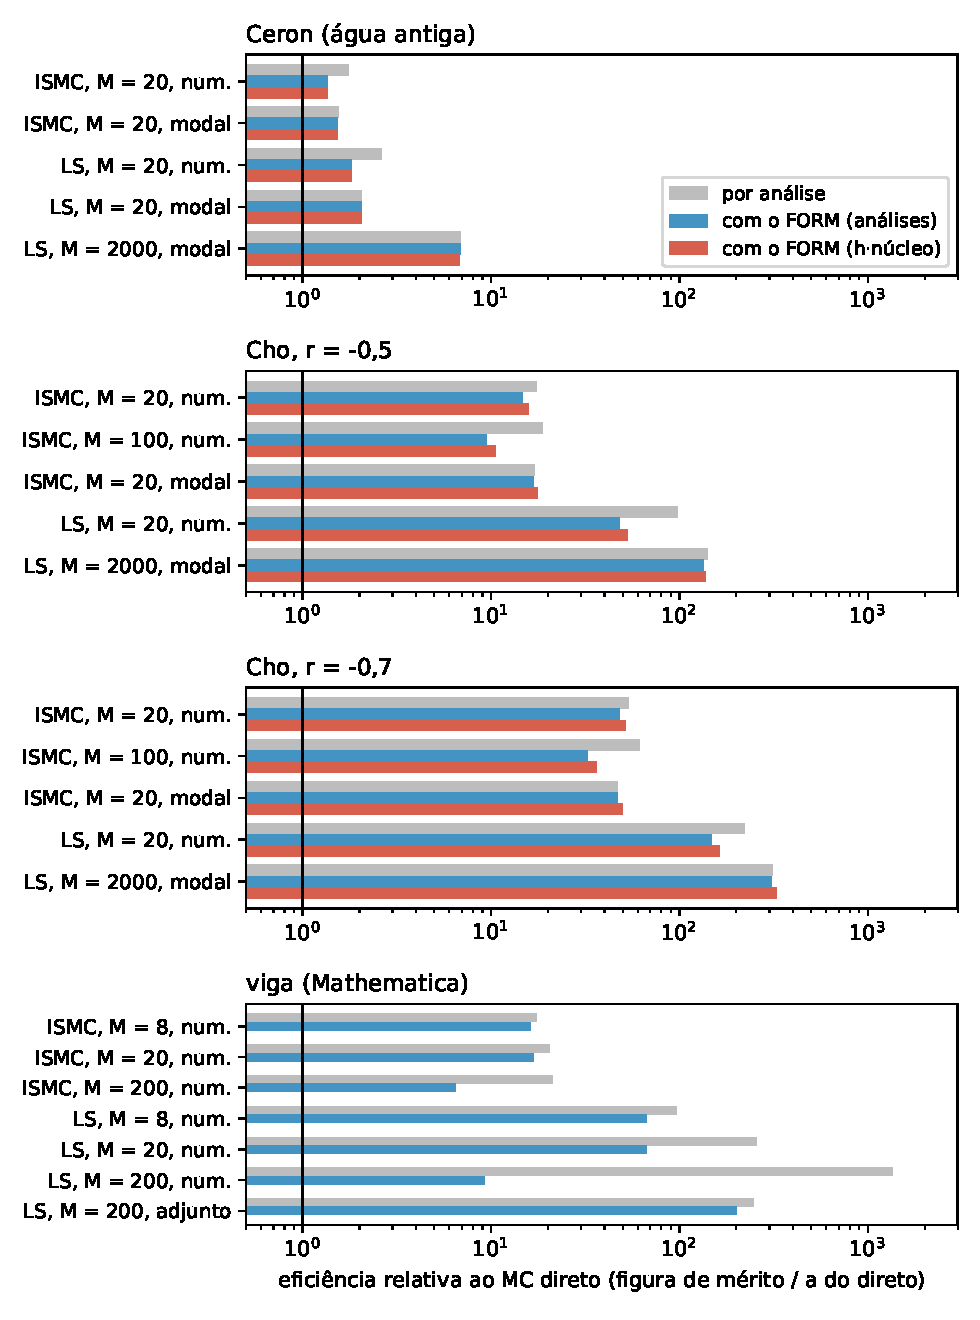
\includegraphics[width=\textwidth]{figs/eficiencia_barras.pdf}
\caption{A eficiência relativa ao Monte Carlo direto (escala logarítmica; 1 = o direto). Cinza: por análise de
amostragem, sem o FORM; azul: com o FORM, em análises; vermelho: com o FORM, em h$\cdot$núcleo (só nos taludes).}
\label{fig:eficbar}
\end{figure}

\section{Diagnósticos da ISMC}\label{sec:ismcdiag}
A Tabela~\ref{tab:ismcdiag} e a Figura~\ref{fig:pesos} olham os pesos $w = e^{-\xib^*\cdot\xib + |\xib^*|^2/2}$.
\begin{itemize}
  \item \textbf{Média dos pesos.} Sob a densidade deslocada, $E[w] = 1$. As médias por semente ficam entre 0,77 e 1,28
    no Cho e perto de 1,1 no Ceron: sem sinal de erro no deslocamento. Na viga, uma das 10 sementes (s110) tem média
    2,37, puxada por um único peso de $\approx 1050$ numa amostra segura (não entra na $P_f$).
  \item \textbf{ESS.} Com todos os pesos, o tamanho efetivo da amostra é pequeno (18 a 109 no Cho, para $N$ de
    1160 a 2990): os pesos das amostras seguras, longe do ponto de projeto, variam muito. Mas esses não entram na $P_f$.
    Só com $I w$, o ESS é \essIwMin{} a \essIwMax\,\% de $N$ no Cho, 22 a 25\,\% no Ceron e uns 30\,\% na viga. Este
    número não é um diagnóstico independente: com a variância amostral, $\mathrm{ESS}(Iw)/N = 1/[1 + (N - 1)\,\mathrm{CoV}^2]
    \approx 1/(1 + \delta_1^2)$, ou seja, é o mesmo $\delta_1$ da Seção~\ref{sec:efic} escrito de outro jeito (por isso
    o ESS$(Iw)$ fica perto de 300 a 400 em todas as sementes do Cho, que pararam com CoV de 5\,\%: $1/0{,}05^2 = 400$).
    O que ele acrescenta é o maior $I w$, que nunca passa de 2\,\% da soma: nenhuma amostra domina a estimativa.
  \item \textbf{Falhas na amostra deslocada:} 42 a 45\,\% no Cho com $r = -0{,}5$, 37 a 40\,\% com $r = -0{,}7$, 48\,\%
    no Ceron e 54\,\% na viga. Perto de 50\,\%, como se espera com o centro no ponto de projeto; um pouco menos no Cho,
    porque a superfície de falha se curva para longe da origem (o FORM superestima a $P_f$: $\Phi(-\beta) = 2{,}4\,\%$ e
    0,68\,\%, contra 1,70 e 0,366\,\% do direto).
  \item \textbf{Os $\ln w$ das falhas} (Figura~\ref{fig:pesos}) ficam abaixo de 0 e numa faixa mais estreita que a
    de todas as amostras, mas ainda larga: no Cho, $\ln w$ vai de uns $-10$ a $-1$ (os $w$ das falhas variam em 3 a 4
    ordens de grandeza). A variância da ISMC vem de duas fontes: metade das amostras não falha (o 0) e os $w$ das que
    falham variam muito. O line sampling elimina as duas, trocando o 0 ou $w$ de cada amostra pela probabilidade exata
    ao longo da linha.
\end{itemize}
% gerado por gera_dados.py
\begin{landscape}
\begin{table}[H]\centering\footnotesize
\caption{Diagnósticos da ISMC, por centro (no Cho, a média das 5 sementes e, entre parênteses, a menor e a maior). $\bar w$: a média dos pesos (deve ficar perto de 1); ESS$(w) = (\sum w)^2/\sum w^2$ com todos os pesos e ESS$(Iw)$ só com os que entram na $P_f$; ``maior'': o maior $I w$ sobre a soma; ``falhas'': a fração da amostra deslocada que falha.}\label{tab:ismcdiag}
\begin{tabular}{llrrrrrr}\toprule
problema & centro & $N$ & $\bar w$ & ESS$(w)$ & ESS$(Iw)$ & maior & falhas \\\midrule
Ceron, rebaixamento & $M = 20$, num. & 1\,000 & 1,12 & 212 & 245 & 1,6\,\% & 48\,\% \\
Ceron, rebaixamento & $M = 20$, modal & 1\,000 & 1,11 & 210 & 223 & 1,9\,\% & 48\,\% \\
Cho, $r = -0{,}5$ & $M = 20$, num. & 1\,350 (1\,250--1\,440) & 1,08 (0,91--1,20) & 62 (34--101) & 313 (305--319) & 1,1 (0,8--1,7)\,\% & 43 (42--44)\,\% \\
Cho, $r = -0{,}5$ & $M = 100$, num. & 1\,254 (1\,160--1\,330) & 1,10 (0,96--1,18) & 59 (35--88) & 307 (299--313) & 1,2 (0,8--1,9)\,\% & 43 (42--44)\,\% \\
Cho, $r = -0{,}5$ & $M = 20$, modal & 1\,400 (1\,290--1\,490) & 1,05 (0,93--1,19) & 69 (44--109) & 317 (309--325) & 1,2 (0,9--1,5)\,\% & 44 (42--45)\,\% \\
Cho, $r = -0{,}7$ & $M = 20$, num. & 2\,104 (2\,000--2\,260) & 1,02 (0,77--1,28) & 41 (18--78) & 347 (340--354) & 1,2 (1,0--1,6)\,\% & 39 (38--40)\,\% \\
Cho, $r = -0{,}7$ & $M = 100$, num. & 1\,818 (1\,730--1\,940) & 1,01 (0,80--1,13) & 38 (18--58) & 336 (333--339) & 1,2 (1,0--1,4)\,\% & 39 (37--40)\,\% \\
Cho, $r = -0{,}7$ & $M = 20$, modal & 2\,498 (2\,190--2\,990) & 0,91 (0,77--1,05) & 53 (36--80) & 369 (351--406) & 1,4 (1,1--1,8)\,\% & 38 (37--40)\,\% \\
viga & $M = 8$, num. & 1000 & 1,10 & 14 & 272 & 1,2\,\% & 54\,\% \\
viga & $M = 20$, num. & 1000 & 1,05 & 23 & 305 & 0,9\,\% & 54\,\% \\
viga & $M = 200$, num. & 1000 & 0,99 & 30 & 313 & 0,9\,\% & 54\,\% \\
viga & $M = 200$, num., 10 sem. & 1\,000 (1\,000--1\,000) & 1,13 (0,80--2,37) & 40 (5--86) & 302 (292--319) & 0,8 (0,7--0,9)\,\% & 53 (52--55)\,\% \\
\bottomrule\end{tabular}\end{table}
\end{landscape}

\begin{figure}[H]\centering
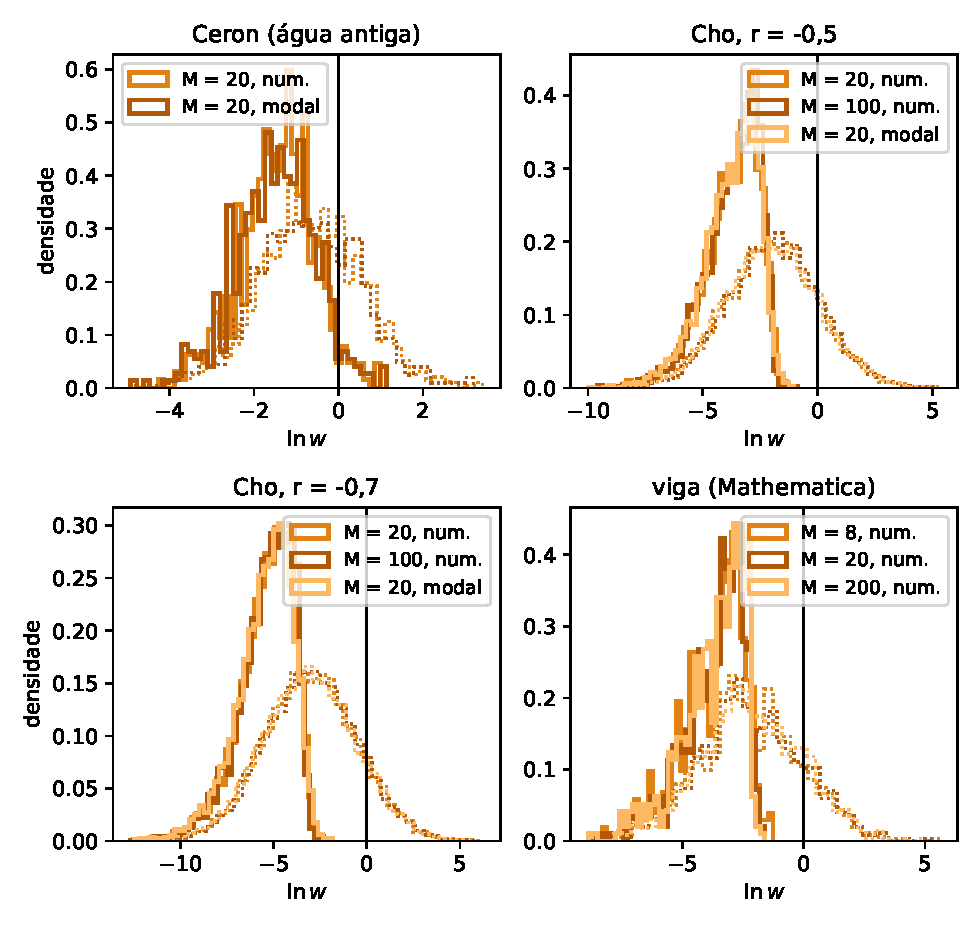
\includegraphics[width=\textwidth]{figs/ismc_pesos.pdf}
\caption{Os pesos da ISMC, $\ln w$, por centro (no Cho, as 5 sementes juntas). Linha cheia: as amostras que falham (as
que entram na $P_f$); pontilhada: todas. As densidades estão normalizadas separadamente.}\label{fig:pesos}
\end{figure}

\section{Diagnósticos do line sampling}\label{sec:lsdiag}
O \texttt{analises.csv} guarda, para cada análise, a linha, o $c$ e o fator ($\Gamma$ ou FS). Com ele, a busca de cada
linha foi refeita com a regra do \texttt{line\_sampling.py}: a 1.ª análise em $c = \beta$, a 2.ª no passo de Newton com a
inclinação $s$, e depois secante, com bissecção só quando a secante sai da cerca. A reconstrução reproduziu todos os
passos gravados (coluna ``conferência'' da Tabela~\ref{tab:lsdiag}).
\begin{itemize}
  \item \textbf{Análises por linha:} 2 ou 3 em quase todas as linhas; 4 ou 5 em poucas (até 8 de 100, no Cho com
    $r = -0{,}7$). Nenhuma linha chegou ao máximo de 10 análises nem aos limites $(-8, 12)$, e não houve $\Gamma = 0$.
  \item \textbf{Secante e bissecção:} todos os passos depois do 2.º foram de secante, exceto uma bissecção em cada
    direção do Cho com $r = -0{,}7$.
  \item \textbf{$\ln(\text{fator})$ ao longo das linhas} (Figura~\ref{fig:lscurvas}): com 2 ou 3 pontos por linha
    não se vê a curvatura na figura; o sinal de que $\ln(\text{fator})$ é quase reto em $c$ é que, em 39 a 78\,\% das linhas dos taludes (98\,\% ou
    mais na viga), a 2.ª análise (o passo de Newton com a inclinação $s$) já cai a menos da tolerância da raiz da
    secante. As linhas com 4 ou 5 análises são as que começam mais longe
    da falha.
  \item \textbf{$\nu_\ell$ e o CoV por linha:} a dispersão de $\nu_\ell$ é o que sobra da variância. Com a direção de
    2000 termos, o CoV de uma linha cai de 90--104\,\% para 59\,\% no Ceron, de 50 para 42\,\% no Cho com $r = -0{,}5$ e de
    68 para 56\,\% com $r = -0{,}7$. Na viga, a direção de 200 termos dá 13\,\%.
  \item \textbf{A inclinação $s$} (2 análises por direção) é parecida nas duas direções de cada problema. Na viga o
    sinal é o contrário porque lá a função de estado é a flecha.
\end{itemize}
% gerado por gera_dados.py
\begin{landscape}
\begin{table}[H]\centering\footnotesize
\caption{Diagnósticos do line sampling. Análises por linha: quantas linhas pararam com 2, 3, 4 e 5 ou mais análises. A busca de cada linha foi reconstruída do \texttt{analises.csv} com a regra do \texttt{line\_sampling.py}: passos depois do 2.º (secante ou bissecção), linhas no máximo de 10 análises, nos limites $(-8, 12)$ e análises com $\Gamma = 0$ (não houve nenhuma). ``Conferência'': passos em que a reconstrução não bate com o $c$ gravado (0 = a regra foi reproduzida). $s$: a inclinação $d\ln(\text{fator})/dc$ no ponto de projeto. A viga só guardou $\nu_\ell$ e as análises por linha.}\label{tab:lsdiag}
\begin{tabular}{llrrrrrrrrrrr}\toprule
problema & direção & $s$ & 2 & 3 & 4 & $\ge 5$ & secante & bissecção & máx./limites & conferência & $\nu$ mín.--máx. & CoV por linha \\\midrule
Ceron (água antiga) & $M = 20$, num. & -0,185 & 49 & 50 & 1 & 0 & 52 & 0 & 0/0 & 0 & -0,16--3,09 & 90\,\% \\
Ceron (água antiga) & $M = 20$, modal & -0,181 & 59 & 41 & 0 & 0 & 41 & 0 & 0/0 & 0 & -0,66--3,35 & 104\,\% \\
Ceron (água antiga) & $M = 2000$, modal & -0,217 & 78 & 22 & 0 & 0 & 22 & 0 & 0/0 & 0 & 0,22--2,20 & 59\,\% \\
Cho, $r = -0{,}5$ & $M = 20$, num. & -0,077 & 70 & 29 & 1 & 0 & 31 & 0 & 0/0 & 0 & 1,67--2,86 & 50\,\% \\
Cho, $r = -0{,}5$ & $M = 2000$, modal & -0,077 & 72 & 25 & 3 & 0 & 31 & 0 & 0/0 & 0 & 1,74--2,86 & 42\,\% \\
Cho, $r = -0{,}7$ & $M = 20$, num. & -0,060 & 45 & 49 & 3 & 3 & 63 & 1 & 0/0 & 0 & 2,23--3,65 & 68\,\% \\
Cho, $r = -0{,}7$ & $M = 2000$, modal & -0,063 & 39 & 53 & 5 & 3 & 71 & 1 & 0/0 & 0 & 2,31--3,97 & 56\,\% \\
viga (Mathematica) & $M = 8$, num. & 0,140 & 488 & 12 & 0 & 0 & -- & -- & -- & -- & 1,38--2,62 & 49\,\% \\
viga (Mathematica) & $M = 20$, num. & 0,142 & 498 & 2 & 0 & 0 & -- & -- & -- & -- & 1,63--2,34 & 30\,\% \\
viga (Mathematica) & $M = 200$, num. & 0,142 & 499 & 1 & 0 & 0 & -- & -- & -- & -- & 1,78--2,18 & 13\,\% \\
viga (Mathematica) & $M = 200$, adjunto & 0,142 & 496 & 4 & 0 & 0 & -- & -- & -- & -- & 1,62--2,31 & 31\,\% \\
\bottomrule\end{tabular}\end{table}
\end{landscape}

\begin{figure}[H]\centering
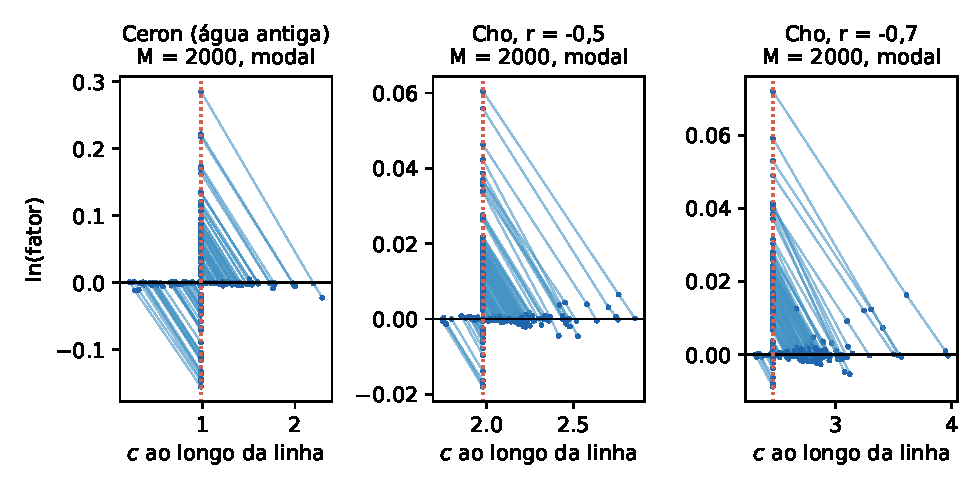
\includegraphics[width=\textwidth]{figs/ls_curvas.pdf}
\caption{$\ln(\text{fator})$ contra $c$ ao longo de cada linha (pontos: as análises; retas: as linhas), na direção do FORM
modal com 2000 termos. Pontilhado vermelho: $c = \beta$, onde toda linha começa. A raiz de cada linha é onde ela cruza o
zero.}\label{fig:lscurvas}
\end{figure}

\section{CoV estimado e CoV observado}\label{sec:covobs}
O CoV que cada método informa vem da variância da própria amostra. Para conferir, é preciso repetir com outras sementes
(Tabela~\ref{tab:covobs}):
\begin{itemize}
  \item \textbf{Cho, ISMC (5 sementes por centro):} com $r = -0{,}5$, o CoV observado entre as sementes, na parada, fica
    entre 0,91 e 1,13 vezes o estimado (5\,\%). Com $r = -0{,}7$, entre 0,47 e 0,58: dentro da faixa de 95\,\% para 5
    sementes (0,35 a 1,67), mas os três centros ficam abaixo. Os três usam as mesmas sementes, então não são três
    conferências independentes; com 5 sementes, o próprio desvio padrão tem erro de uns $\pm 35\,\%$. Pode ser acaso ou
    um CoV estimado um pouco conservador; não dá para separar com estes dados.
  \item \textbf{Viga, ISMC (10 sementes independentes, centro do FORM $M = 200$):} razão de 0,77, dentro da faixa
    (0,55 a 1,45).
  \item \textbf{Line sampling e Ceron:} uma semente só por direção ou centro; o CoV observado entre sementes não existe
    ainda (pendência).
  \item \textbf{Cobertura:} o intervalo de 95\,\% de cada semente da ISMC (Cho e viga) contém a $P_f$ do direto em
    \icDentro{} de \icTotal{} casos, e todas as \zTotal{} estimativas (sementes da ISMC, ISMC do Ceron, line sampling)
    têm $|z| < 1{,}96$ contra o direto (Figura~\ref{fig:z}). O desvio quadrático médio dos $z$ é \zSd, abaixo de 1: o
    $z$ inclui o erro do direto, que é o mesmo para todas as estimativas de um problema, e as sementes são comuns aos
    centros. Esperava-se uns 5\,\% fora; nenhum fora é coerente com um CoV estimado correto ou um pouco conservador.
  \item \textbf{A parada pelo CoV} (Tabela~\ref{tab:parada}): a $P_f$ na parada difere da $P_f$ com todas as realizações
    da semente em \viesParada\,\% na média (de \viesParadaMin{} a \viesParadaMax\,\% por semente): o viés da parada
    opcional não aparece, como esperado (ordem de $\mathrm{CoV}^2$).
  \item \textbf{Bases diferentes:} os diretos do Cho usam a KL com variância retida de 0,9877 e as ISMC e o line
    sampling, a base de Nyström de 2000 modos com 0,9973. As $P_f$ batem dentro do ruído ($|z| \le 0{,}75$), então a
    diferença não aparece nesta precisão.
\end{itemize}
% gerado por gera_dados.py
\begin{table}[H]\centering\footnotesize
\caption{O CoV estimado contra o observado entre sementes. Cho: as 5 sementes de cada centro, na parada (o $N$ do arquivo \texttt{ATINGIU}); viga: 10 sementes de 1000 amostras com o centro do FORM $M = 200$. Se o CoV estimado está certo, a razão observado/estimado cai, com 95\,\% de chance, na faixa da última coluna ($\sqrt{\chi^2_{k-1}/(k-1)}$).}\label{tab:covobs}
\begin{tabular}{llrrrrrrr}\toprule
caso & centro da ISMC & sem. & $N$ médio & $P_f$ média & \makecell{CoV\\estimado} & \makecell{CoV\\observado} & razão & \makecell{faixa\\de 95\,\%} \\\midrule
Cho, $r = -0{,}5$ & $M = 20$, num. & 5 & 1\,334 & 1,749\,\% & 5,0\,\% & 4,5\,\% & 0,91 & 0,35--1,67 \\
Cho, $r = -0{,}5$ & $M = 100$, num. & 5 & 1\,240 & 1,752\,\% & 5,0\,\% & 5,6\,\% & 1,13 & 0,35--1,67 \\
Cho, $r = -0{,}5$ & $M = 20$, modal & 5 & 1\,380 & 1,718\,\% & 5,0\,\% & 4,8\,\% & 0,96 & 0,35--1,67 \\
Cho, $r = -0{,}7$ & $M = 20$, num. & 5 & 2\,050 & 0,363\,\% & 5,0\,\% & 2,9\,\% & 0,58 & 0,35--1,67 \\
Cho, $r = -0{,}7$ & $M = 100$, num. & 5 & 1\,786 & 0,361\,\% & 5,0\,\% & 2,5\,\% & 0,51 & 0,35--1,67 \\
Cho, $r = -0{,}7$ & $M = 20$, modal & 5 & 2\,310 & 0,354\,\% & 5,0\,\% & 2,4\,\% & 0,47 & 0,35--1,67 \\
viga & $M = 200$, num. & 10 & 1\,000 & 2,115\,\% & 4,8\,\% & 3,7\,\% & 0,77 & 0,55--1,45 \\
\bottomrule\end{tabular}\end{table}
\begin{table}[H]\centering\footnotesize
\caption{A parada pelo CoV na ISMC do Cho: a $P_f$ na parada contra a $P_f$ com todas as realizações da mesma semente (os blocos que já rodavam terminaram depois da parada).}\label{tab:parada}
\begin{tabular}{llrrrr}\toprule
caso & centro & $N$ na parada & $N$ com tudo & $P_f$ na parada & $P_f$ com tudo \\\midrule
Cho, $r = -0{,}5$ & $M = 20$, num. & 6\,670 & 6\,750 & 1,749\,\% & 1,743\,\% \\
Cho, $r = -0{,}5$ & $M = 100$, num. & 6\,200 & 6\,270 & 1,752\,\% & 1,749\,\% \\
Cho, $r = -0{,}5$ & $M = 20$, modal & 6\,900 & 7\,000 & 1,718\,\% & 1,721\,\% \\
Cho, $r = -0{,}7$ & $M = 20$, num. & 10\,250 & 10\,520 & 0,363\,\% & 0,365\,\% \\
Cho, $r = -0{,}7$ & $M = 100$, num. & 8\,930 & 9\,090 & 0,361\,\% & 0,363\,\% \\
Cho, $r = -0{,}7$ & $M = 20$, modal & 11\,550 & 12\,490 & 0,354\,\% & 0,351\,\% \\
\bottomrule\end{tabular}\end{table}

\begin{figure}[H]\centering
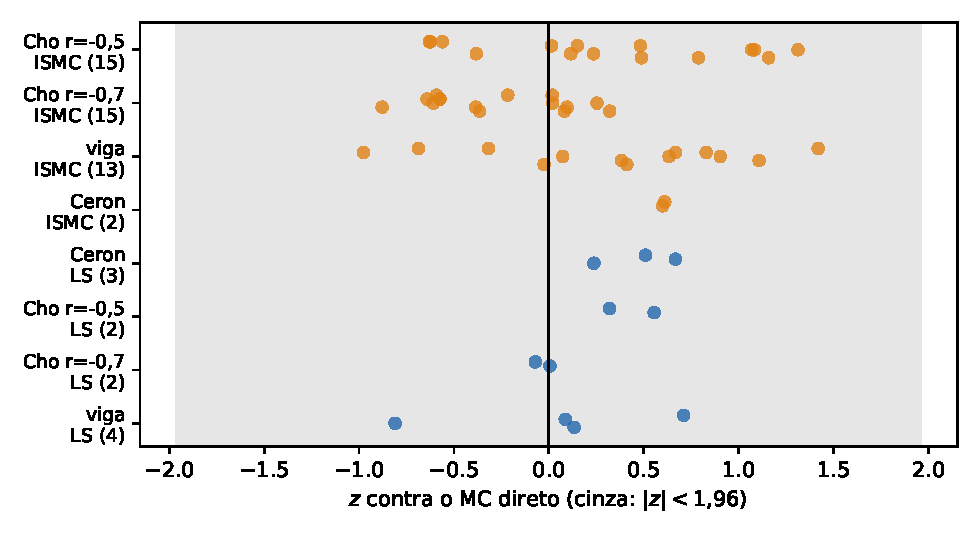
\includegraphics[width=\textwidth]{figs/z_todos.pdf}
\caption{O $z$ de cada estimativa contra o Monte Carlo direto do mesmo problema. Laranja: ISMC (no Cho e na viga, uma
semente por ponto, na parada); azul: line sampling. Entre parênteses, quantas estimativas.}\label{fig:z}
\end{figure}

\section{Tabela-síntese}\label{sec:tabsint}
A Tabela~\ref{tab:sintese} junta, por problema e método, as métricas das seções anteriores.
% gerado por gera_dados.py
\begin{landscape}
\begin{table}[p]\centering\footnotesize\setlength{\tabcolsep}{4pt}
\caption{Tabela-síntese: todas as métricas por método e problema. FORM: iterações/análises. $n$: análises da amostragem já feitas. $\delta_1$: o CoV de uma análise. $N_5$: análises para CoV de 5\,\%, com o FORM; $H_5$: as h$\cdot$núcleo correspondentes (Tabela~\ref{tab:tempo}; a viga só por análises). Efic.: a eficiência relativa ao direto, por análise de amostragem / com o FORM / em tempo. Diagnóstico: ESS$(Iw)/N$ na ISMC, análises por linha no LS. Na ISMC da viga, $N_5$ usa o CoV estimado da rodada (na Tabela~\ref{tab:viga}, o CoV calculado com o direto).}\label{tab:sintese}
\begin{tabular}{lllrrrrrrrrrl}\toprule
problema & método & centro/direção & FORM & $n$ & $P_f$ & CoV & $z$ & $\delta_1$ & $N_5$ & $H_5$ (h) & efic. & diagnóstico \\\midrule
Ceron (água antiga) & MC direto & -- & -- & 2\,000 & 15,700\,\% & 5,2\,\% & -- & 2,32 & 2\,148 & 21,3 & 1,0/1,0/1,0 & -- \\
 & ISMC & $M = 20$, num. & 3/363 & 1\,000 & 16,447\,\% & 5,6\,\% & 0,61 & 1,76 & 1\,595 & 15,8 & 1,7/1,3/1,3 & ESS(Iw)/N = 25\,\% \\
 & ISMC & $M = 20$, modal & 3/3 & 1\,000 & 16,460\,\% & 5,9\,\% & 0,60 & 1,87 & 1\,397 & 13,9 & 1,5/1,5/1,5 & ESS(Iw)/N = 22\,\% \\
 & LS (100 lin.) & $M = 20$, num. & 3/363 & 254 & 16,566\,\% & 9,0\,\% & 0,51 & 1,44 & 1\,183 & 11,7 & 2,6/1,8/1,8 & 2,52 an./linha \\
 & LS (100 lin.) & $M = 20$, modal & 3/3 & 243 & 16,998\,\% & 10,4\,\% & 0,67 & 1,62 & 1\,046 & 10,4 & 2,0/2,1/2,0 & 2,41 an./linha \\
 & LS (100 lin.) & $M = 2000$, modal & 3/3 & 224 & 15,996\,\% & 5,9\,\% & 0,24 & 0,88 & 313 & 3,1 & 6,9/6,9/6,8 & 2,22 an./linha \\
\midrule
Cho, $r = -0{,}5$ & MC direto & -- & -- & 24\,000 & 1,700\,\% & 4,9\,\% & -- & 7,60 & 23\,129 & 444,7 & 1,0/1,0/1,0 & -- \\
 & ISMC (5 sem.) & $M = 20$, num. & 3/243 & 6\,750 & 1,740\,\% & 2,2\,\% & 0,43 & 1,82 & 1\,570 & 28,3 & 17,4/14,7/15,7 & ESS(Iw)/N = 23\,\% \\
 & ISMC (5 sem.) & $M = 100$, num. & 3/1203 & 6\,270 & 1,745\,\% & 2,2\,\% & 0,49 & 1,76 & 2\,439 & 42,2 & 18,7/9,5/10,5 & ESS(Iw)/N = 24\,\% \\
 & ISMC (5 sem.) & $M = 20$, modal & 10/10 & 7\,000 & 1,718\,\% & 2,2\,\% & 0,19 & 1,85 & 1\,375 & 25,1 & 16,9/16,8/17,7 & ESS(Iw)/N = 23\,\% \\
 & LS (100 lin.) & $M = 20$, num. & 3/243 & 233 & 1,739\,\% & 5,0\,\% & 0,32 & 0,77 & 480 & 8,4 & 97,6/48,2/53,1 & 2,31 an./linha \\
 & LS (100 lin.) & $M = 2000$, modal & 7/7 & 233 & 1,762\,\% & 4,2\,\% & 0,56 & 0,64 & 172 & 3,2 & 141,1/134,8/138,0 & 2,31 an./linha \\
\midrule
Cho, $r = -0{,}7$ & MC direto & -- & -- & 110\,000 & 0,366\,\% & 5,0\,\% & -- & 16,49 & 108\,781 & 2\,061,5 & 1,0/1,0/1,0 & -- \\
 & ISMC (5 sem.) & $M = 20$, num. & 3/243 & 10\,520 & 0,366\,\% & 2,2\,\% & -0,04 & 2,25 & 2\,270 & 39,7 & 53,5/47,9/52,0 & ESS(Iw)/N = 16\,\% \\
 & ISMC (5 sem.) & $M = 100$, num. & 4/1604 & 9\,090 & 0,362\,\% & 2,2\,\% & -0,20 & 2,10 & 3\,369 & 57,1 & 61,5/32,3/36,1 & ESS(Iw)/N = 18\,\% \\
 & ISMC (5 sem.) & $M = 20$, modal & 8/8 & 12\,490 & 0,352\,\% & 2,2\,\% & -0,75 & 2,41 & 2\,310 & 41,1 & 46,9/47,1/50,1 & ESS(Iw)/N = 15\,\% \\
 & LS (100 lin.) & $M = 20$, num. & 3/243 & 266 & 0,364\,\% & 6,8\,\% & -0,07 & 1,11 & 732 & 12,6 & 221,9/148,7/163,7 & 2,64 an./linha \\
 & LS (100 lin.) & $M = 2000$, modal & 5/5 & 274 & 0,367\,\% & 5,6\,\% & 0,01 & 0,93 & 353 & 6,3 & 311,7/307,8/327,3 & 2,72 an./linha \\
\midrule
viga (Mathematica) & MC direto & -- & -- & 50\,000 & 2,098\,\% & 3,1\,\% & -- & 6,83 & 18\,666 & -- & 1,0/1,0/-- & -- \\
 & ISMC & $M = 8$, num. & 4/85 & 1\,000 & 2,289\,\% & 5,2\,\% & 1,42 & 1,64 & 1\,157 & -- & 17,4/16,1/-- & ESS(Iw)/N = 27\,\% \\
 & ISMC & $M = 20$, num. & 4/205 & 1\,000 & 2,200\,\% & 4,8\,\% & 0,83 & 1,51 & 1\,116 & -- & 20,5/16,7/-- & ESS(Iw)/N = 31\,\% \\
 & ISMC & $M = 200$, num. & 4/2005 & 1\,000 & 2,208\,\% & 4,7\,\% & 0,90 & 1,48 & 2\,884 & -- & 21,2/6,5/-- & ESS(Iw)/N = 31\,\% \\
 & LS (500 lin.) & $M = 8$, num. & 4/85 & 1\,014 & 2,155\,\% & 2,2\,\% & 0,71 & 0,70 & 281 & -- & 96,1/66,5/-- & 2,02 an./linha \\
 & LS (500 lin.) & $M = 20$, num. & 4/205 & 1\,004 & 2,104\,\% & 1,3\,\% & 0,09 & 0,43 & 280 & -- & 256,9/66,8/-- & 2,00 an./linha \\
 & LS (500 lin.) & $M = 200$, num. & 4/2005 & 1\,003 & 2,045\,\% & 0,6\,\% & -0,81 & 0,19 & 2\,021 & -- & 1\,351,9/9,2/-- & 2,00 an./linha \\
 & LS (500 lin.) & $M = 200$, adjunto & 4/15 & 1\,006 & 2,107\,\% & 1,4\,\% & 0,13 & 0,43 & 92 & -- & 246,8/201,8/-- & 2,01 an./linha \\
\bottomrule\end{tabular}\end{table}
\end{landscape}


\section{Síntese}
\begin{enumerate}
  \item \textbf{Nenhum viés detectado.} Nos taludes, $|z| \le \zMaxTaludes$ em todos os métodos (Tabelas~\ref{tab:ceron} a
    \ref{tab:r07}); na viga, o maior é o da ISMC com o centro do FORM $M = 8$, $z = 1{,}42$ (relatório da viga), dentro da
    flutuação esperada. As cinco sementes de cada ISMC se espalham em torno do direto (Figura~\ref{fig:sementes}). As
    três ISMC de cada caso usam as mesmas sementes (números aleatórios comuns), então os seus erros andam juntos (com
    $r = -0{,}5$, a semente 21 é a mais baixa nos três centros): não são três conferências independentes, mas a comparação entre os
    centros fica mais justa. O line sampling tem uma semente só.
  \item \textbf{O line sampling com a direção do FORM modal de todos os modos foi o mais barato em todos os taludes:}
    \lsNCe{} análises no Ceron, \lsNRa{} no Cho $r = -0{,}5$ e \lsNRb{} no Cho $r = -0{,}7$, isto é, \lsGanhoCe, \lsGanhoRa{}
    e \lsGanhoRb{} vezes menos que o direto, e \lsGanhoIsmcCe, \lsGanhoIsmcRa{} e \lsGanhoIsmcRb{} vezes menos que a melhor
    ISMC. O FORM modal custa uma análise por iteração (3 a 10 análises nos três taludes; 3 a 7 com todos os modos), e esse
    custo não cresce com o número de termos.
  \item \textbf{A direção precisa dos modos altos quando a ruptura passa por bandas fracas locais} (Ceron): com 20 termos
    por campo, o line sampling custa $\approx 1050$ a 1180 análises; com 2000, \lsNCe. No Cho, em que a falha depende
    dos primeiros modos de $\varphi'$, o $\beta$ quase não muda com os modos altos (Tabela~\ref{tab:form}).
  \item \textbf{Na ISMC, o centro do FORM com $M = 100$ não compensa:} melhora pouco a amostragem e custa 1200 a 1600
    análises de FORM. O centro modal com 20 termos (8 a 10 análises) empata com o numérico (243).
  \item \textbf{Viga:} o mesmo padrão; com a direção do gradiente adjunto (200 termos, 15 análises), o line sampling dá
    CoV de 5\,\% com 92 análises, contra 18\,666 do direto.
  \item \textbf{Em h$\cdot$núcleo, o quadro é o mesmo} (Seção~\ref{sec:tempo}): o custo de uma análise quase não muda
    entre os métodos, e o FORM modal é barato (0,06 a 0,2 h, mesmo com a parede do gradiente modal). Para CoV de 5\,\%
    no Cho com $r = -0{,}7$: \hDirRb{} h no direto, \hIsmcRb{} na melhor ISMC e \hLsRb{} no line sampling modal; a
    etapa 3b inteira (30 ISMC) gastou \hIsmcTotal{} h$\cdot$núcleo.
  \item \textbf{Por análise, o line sampling rende uns 5 a 8 vezes a ISMC no Cho} (Seção~\ref{sec:efic}):
    $\delta_1 \approx 0{,}6$ a 1,1 contra 1,8 a 2,4, e a razão $(\delta_{1,\text{ISMC}}/\delta_{1,\text{LS}})^2$ é
    \lsIsmcMelhorRa{} ($r = -0{,}5$) e \lsIsmcMelhorRb{} ($r = -0{,}7$) entre o melhor de cada método (\lsIsmcMin{} a
    \lsIsmcMax{} entre todos os pares de centro e direção). O FORM numérico com muitos termos pode desfazer essa vantagem (viga, $M = 200$).
  \item \textbf{Os diagnósticos não mostram problema}: médias dos pesos perto de 1 e nenhum peso dominante (o maior
    $I w$ fica abaixo de 2\,\% da soma); no line sampling, nenhuma linha nos limites ou no máximo de análises, e só 2 bissecções em 700
    linhas dos taludes.
  \item \textbf{O CoV estimado é confiável ou um pouco conservador} (Seção~\ref{sec:covobs}): nas ISMC, o CoV observado
    entre sementes fica entre 0,47 e 1,13 vezes o estimado, sempre dentro da faixa de 95\,\%; todos os intervalos
    contêm a $P_f$ do direto, e a parada pelo CoV não deixa viés visível.
  \item \textbf{O SRM e o GIM dão a mesma $P_f$} (Seção~\ref{sec:pareado}, ISMC do GIM parcial): nas mesmas
    realizações e nas mesmas linhas, a diferença é de no máximo \sgDifAbsMax\,\%, com o GIM um pouco abaixo (na ISMC, só
    por realizações limítrofes), dentro do CoV de cada estimativa; o GIM é \sgEcon\,\% mais barato por análise (no line
    sampling, empata por linha). No Ceron com a água do artigo, o line sampling do MEF dá \ceaLsPf, contra \ceaPfArt{}
    do artigo (Seção~\ref{sec:ceronagua}).
\end{enumerate}
Decisão (20/11/2026): o line sampling na direção do FORM modal com todos os modos é o método padrão, com a ISMC como
conferência, até que se prove o contrário.

\section{Pendências}
\begin{itemize}
  \item O line sampling não grava o tempo de cada análise (apaga os CSV): guardar \texttt{s\_fator} no
    \texttt{analises.csv}, para medir o custo em vez de estimá-lo. O mesmo para o número de \emph{kernels} na viga.
  \item A CPU oficial dos jobs da etapa 3b (o \texttt{TotalCPU} do \texttt{sacct} dos jobs 14891 a 14894) não está
    no PC; aqui a CPU é a soma de \texttt{s\_fator}.
  \item No Ceron, a ISMC também tem uma semente só por centro.
  \item Repetir o line sampling com 2 ou 3 sementes num caso (Cho $r = -0{,}7$) para conferir o CoV estimado pelas linhas
    contra a dispersão entre sementes.
  \item Chuva: o line sampling ainda não foi testado; a direção modal não tem componente em $k_s$ e pode haver mais de um
    mecanismo no tempo (formulação, Seção do line sampling, passo 8).
  \item Completar a comparação pareada da Seção~\ref{sec:pareado} quando o fermi terminar (o GIM até 2000 realizações
    por caso e a coluna da análise limite, jobs 14991 e 14992) e entender por que a análise limite em Python dá
    \ceaMcPfEx{} no Ceron com a água do artigo, contra \ceaPfArt{} do artigo.
\end{itemize}
\end{document}
